% !TeX root = ../thuthesis-example.tex

\chapter{补充内容}


\section{综述补充}
  \subsection{模块化自动驾驶} 
  \label{sub:pipeline}
    近年来模块化路线的一个共同趋势是\emph{预测--决策一体化}：将自车决策作为条件变量，显式或隐式地建模“自车动作$\rightarrow$他车响应”的耦合关系，并在候选决策之间做综合评估。现有研究大体可按交互处理方式划分为显式交互、隐式交互及综合式交互三类。

    \emph{显式交互}以自车候选策略/意图划分场景，在每个候选行为下预测周车反应，并对不同候选行为的长期收益与风险进行比较，典型代表为多策略决策方法（Multi-Policy Decision Method, MPDM）。Cunningham等\cite{cunningham2015mpdm,galceran2017changepoint}提出MPDM思想，将交互不确定性建模为部分可观测马尔可夫决策过程（Partially Observable Markov Decision Problem, POMDP），并用一组闭环策略/意图近似描述自车与周车的决策空间，从而显著压缩搜索规模。Ding等提出的EPSILON\cite{ding2022epsilon}继承并改进该思想，提出领域特定闭环策略树（Domain-Specific-Policy Tree, DCP-Tree）与条件集中分支（Conditional Focused Branching, CFB）机制\cite{zhang2020guidedbranching}，通过限制自车策略展开深度并聚焦意图不确定性高的周车，提升了在线规划的效率；并进一步结合时空语义走廊规划器\cite{ding2019semanticcorridor}用于运动规划。Bae等\cite{bae2023lanechange}结合MPC与生成对抗网络（Generative Adversarial Network, GAN）生成平滑换道轨迹，并引入自适应安全边界与卡尔曼滤波以提升密集交通中的鲁棒性与可用性。

    \emph{隐式交互}侧重对周车意图/不确定性构造多个可能情景，并在情景集合上评估自车应对策略，典型代表包括防御性规划（Contingency Planning）\cite{salvado2016contingency}与博弈论方法。Huang等\cite{huang2021riskbudget}提出基于风险预算的递归控制算法，通过动态分配风险预算在满足安全约束的同时减少过度保守。Da等\cite{da2022reactivesafety}提出综合反应式安全（Comprehensive Reactive Safty, CRS）框架，强调规划不必在所有未来情形下“绝对无碰撞”，而应能对环境变化做出反应并保证安全，并在此基础上提出反应式迭代线性二次规划（iterative Linear Quadratic Regulator, iLQR）算法。博弈论思路方面，Le Cleach等\cite{li2018gametheoryacc}提出基于无迹卡尔曼滤波的逆动力学博弈用于在线估计其他智能体目标函数，并将其整合到滚动时域博弈规划器中；进一步在\cite{li2020gametheorytits}提出增广拉格朗日快速求解器ALGAMES以求解含非线性约束的多玩家动态博弈问题。Li等\cite{lecleach2020lucidgames}提出面向无信号交叉口的多车博弈框架，并在\cite{lecleach2022algames}提出基于Level-K博弈论的长时域、多步交互决策模型，体现了“交互可解释、决策可推演”的特点。

    \emph{综合式交互}将显式交互与隐式交互思想融合，并常与风险度量、礼貌性或协同性等机制结合。Tong Li等\cite{li2023marc}提出风险敏感多策略防御性规划（Multipolicy and Risk-Aware Contingency Planning, MARC）框架，集成MPDM与风险感知的防御性规划，并通过场景级动态分支点与LP-iLQR双层迭代优化显著提升复杂交互环境下的决策效率与自然性。此外，Sun等\cite{sun2018courteous}在目标函数中引入“对他车成本影响”的度量以形成更礼貌的驾驶行为；Sheng等\cite{sheng2023cooperationaware}利用时空图卷积网络构建交互式轨迹预测模型，用于评估他车对自车决策的反应，从而增强协同意识。


  \subsection{端到端自动驾驶}
    \label{sub:end2end}
    自2022年大语言模型（Large Language Model, LLM）快速兴起以来\cite{AttnIsAllYouNeed2017}，大规模数据驱动的统一表征与跨模态知识融合显著加速了自动驾驶从“模块化流水线”向“可微统一优化”的范式迁移。端到端（End-to-end, E2E）自动驾驶因此成为热点：其核心目标是缓解模块化方案中感知误差难以被后续模块正确吸收、感知—规控接口造成的信息裁剪与不确定性丢失等问题。围绕可微边界的不同，现有端到端路线通常划分为两段式端到端（以结构化感知结果为输入）与一段式端到端（从原始或近原始感知表征直接到规划/控制输出），并进一步发展到“感知直接到控制”的视觉语言动作模型（Vision Language Action Model, VLA）形态。

    两段式端到端通常以结构化感知结果作为输入，是早期端到端方案的主流工程选择，其方法谱系主要包括模仿学习与强化学习，并常组合使用：通过行为克隆、逆最优控制、知识蒸馏等模仿学习\cite{chen2023endtoend}注入先验以快速初始化，再衔接强化学习提升长时域闭环性能。规划挑战体系中，PlanTF\cite{PlanTF2023}奠定了两段式端到端规划的Transformer化范式；PLUTO\cite{PLUTO2024}作为其后续代表，将自车、周车、静态障碍物、静态地图与动态交通信息分路编码，并设计可微辅助任务与横纵向交叉因式分解注意力解码机制，配合规则后处理在综合指标上显著提升表现，首次击败了规则方案：2023年nuPlan挑战赛冠军PDM-Close。CarPlanner\cite{CarPlanner2025}在此基础上引入动作模式一致性的自回归世界模型以增强长时域一致性。与此同时，“将驾驶行为离散化为token并借鉴语言建模训练范式”的路线也被用于两段式体系增强：Wayformer\cite{Wayformer2022}与Trajeglish\cite{Trajeglish2024}体现将自车动作/轨迹离散成“词”的建模思路，Plan-R1\cite{PlanR12025}进一步将强化学习与PLUTO式框架衔接以提升闭环决策质量。总体而言，两段式端到端的优势是输入结构化、跨平台迁移友好、较少面临原始感知域的Sim2Real适配；但其不可避免受限于感知到规控的信息接口，感知不确定性难以在端到端训练中被充分吸收并转化为更优决策，这构成其相对于一段式路线的主要性能上限来源。

    一段式端到端的关键差异在于：规划/决策损失的梯度可以回传到上游感知表征，从而实现感知—预测—决策—规划的整体协同优化。向Transformer迁移的统计基座表征、多模态融合与BEV化输入是端到端方案发展的重要基石。Transformer\cite{AttnIsAllYouNeed2017}奠定了序列建模与注意力机制的通用范式，并促成视觉领域从CNN主导向Transformer主导的快速迁移：ViT\cite{ViT2021}提供视觉Transformer的基础表征框架，DETR\cite{DETR2020}将检测任务显式序列化并实现端到端集合预测，Deformable DETR\cite{Deformable_DETR2021}进一步通过可变形注意力提升稀疏采样效率与收敛质量；相较之下，Faster R-CNN\cite{Faster_RCNN2016}、Mask R-CNN\cite{MaskRCNN2018}与早期YOLO\cite{YOLOv12016}代表传统两阶段/实例分割/单阶段检测范式，在统一序列接口与全局注意力建模方面存在结构性差异。多模态端到端方面，Transfuser\cite{Transfuser2023}代表性地推进了相机/激光雷达等多源原始数据的融合机制，使“在统一表征上直接学习规划”更具工程可行性。纯视觉端到端则普遍以鸟瞰图（Bird-Eye View, BEV）作为统一几何坐标系：Lift-Splat-Shoot\cite{LSS_Lift_Splat_Shoot_BEV2020}提供从图像到BEV的显式几何投影范式，PanopticSegFormer\cite{PanopticSegFormer2022}推进了BEV语义与全景理解能力，BEVFormer\cite{BevFormer2022}进一步通过时序注意力与多相机对齐强化动态场景表征（BEV发展脉络可由\cite{LSS_Lift_Splat_Shoot_BEV2020,PanopticSegFormer2022,BevFormer2022}串联）。在BEV之上，结构化输出同样快速演进：MapTR\cite{MapTR2023}体现BEV到矢量化地图/车道拓扑要素的生成路径，SurroundOcc\cite{SurrondOcc2023}代表占用/可通行空间的体素化建模方向，CASPFormer\cite{CASPFormer2024}则延续以统一Transformer骨干推动多任务场景级理解的一体化趋势。UniAD\cite{hu2022uniAD}与VAD\cite{jiang2023vad}是早期代表：其将检测、跟踪、建图/占用等感知子任务与规划模块网络化并联合训练，使规划学习能够直接利用可学习的中间表征。UAD\cite{guo2024UAD}进一步强调将多模块融合为更统一的综合式架构，并引入无监督预训练以降低对标注的依赖。SparseDrive\cite{SparseDrive2024}体现以更稀疏/关键要素的表示与更高效的推理路径支撑端到端规划，而VADv2\cite{VADv2_2024}则作为VAD体系的重要迭代，强调在训练机制与闭环表现上的增强。在“开环规划/评测”语境下，BEV-Planner\cite{li2024bev_planner}具有代表性：其系统性分析开环端到端评测中的关键细节，并突出自车状态（ego status）在规划学习中的作用，通过面向自车信息的设计改善收敛与鲁棒性，从而为后续端到端规划的输入建模与指标解读提供了可复用的基线框架。在数据来源与目标形式上，Hydra-MDP\cite{li2024hydramdp}采用多模态、多目标的训练范式，将交互逻辑不仅从人类驾驶数据学习，也通过仿真数据补充多样性与长尾覆盖，从而提升端到端规划在稀有工况下的鲁棒性。强化学习与世界模型亦被用于增强闭环能力，例如SEM2\cite{gao2022sem2_worldmodel}通过语义掩码构建世界模型并配合多源采样提高长尾工况比例，体现“以可控数据分布塑形闭环策略”的路线。

    随着端到端从“输出单一最优轨迹”转向“建模可行多模态轨迹分布”，生成式规划成为重要方向。扩散模型体系由去噪扩散概率模型（Denoising Diffusion Probabilistic Model, DDPM）\cite{DDPM2020}奠基，扩散去噪隐式模型（Denoising Diffusion Implicit Model, DDIM）\cite{DDIM2022}提供更快的隐式采样路径大大加速了采样耗时的DDPM，Score-based扩散\cite{Score_based_Diff2021}进一步提供了基于分数函数的训练视角；在数值加速方面，清华大学提出的DPM-Solver系列\cite{DMP_Solver2022,DPM_Solver_v3_2023, DPM_Solver_pp_2024}对高质量加速提供了更好的方案；在更加高维的向量空间表征上，潜空间扩散模型（Latent Diffusion Model, LDM）\cite{LDM_VQGANandDDPM2022}将向量量化生成对抗式网络（Vector Quantised-GAN, VQ-GAN）\cite{VQ_GAN2021}与DDPM结合从而“在潜空间进行扩散”以显著降低生成成本。面向自动驾驶闭环规划，DiffusionPlanner\cite{DiffusionPlanner2025}代表将扩散用于闭环规划并支持预测—规划联合建模的路线，通过生成多模态行为分布提升交互一致性与轨迹质量（并强调减少规则后处理依赖）。相比于传统扩散方式，Flow Matching\cite{FlowMatching2023original}这一条技术路线则提供另一条直接建模概率扩散的方式，建立线性插值的最短路径：“整合流（Rectified Flow）”用于以更少步数实现高效生成。扩散模型跨模态条件生成的范式如DALLE2中CLIP\cite{CLIP2021}与扩散模型结合\cite{DALLE_2_CLIPandDDPM2022}所体现的“条件对齐表征 + 生成模型”框架，并被更新的自动驾驶规划工作用于将地图/交通体/导航意图等条件注入生成过程。在更近期的结果汇总中，DiffusionDrive-v2\cite{DiffusionDrive_v2_2025}引入强化学习约束的截断扩散生成策略，并在其公开报告中给出了在NAVSIM基准上的更高分数，从而在同类生成式规划对比中形成新的强参考点；该结果在文中被表述为当时的基准最优，并体现出对以GoalFlow\cite{GoalFlow2025}为代表的先前强方法的进一步提升。

  \subsection{半侧翻模态及其可控性} 
    \label{sub:semirollover}
    如图~\ref{fig:rollover_modes}所示，车辆侧翻有全部车轮着地模态（未侧翻模态）和一侧车轮离地（半侧翻模态，Semi-Rollover）两种状态\cite{wanying2020antirolover}，而半侧翻模态在很多研究中已经被定义为侧翻。但实际车辆行驶过程中由于操作不慎、绊倒性侧翻等原因在达到半侧翻态时仍旧有将车辆救回的余地。

    \begin{figure}
      \centering
      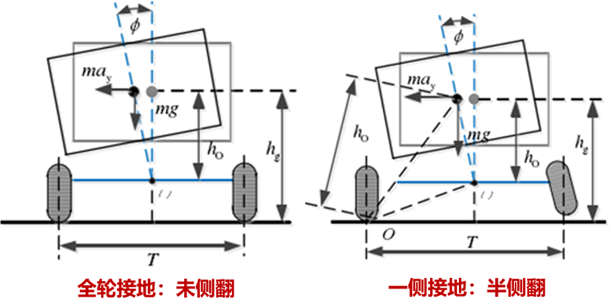
\includegraphics[width=0.7\linewidth]{fig/chap1/rollover_modes.png}
      % \caption*{图片注释解释说明}
      \caption{车辆侧翻的两种模态}
      \label{fig:rollover_modes}
    \end{figure} 

    但由于目前研究只关注未侧翻模态，而忽略了半侧翻模态，国内外缺乏对于半侧翻模态可控性、动力学特性与控制方法的探究，故对吉尼斯记录、网络公开可访问的交通录像资料与影视素材进行了搜索，对该模态的说法一般为侧两轮行驶（Driving on Two Wheels），或单边行驶。首先关注半侧翻模态的发生条件。如图~\ref{fig:semi_rollover_condition}所示，半侧翻状态在小型车辆行驶时一般不容易被动发生，通常是驾驶员认为主动在高速情况下通过ABA式（ABA表示向某向打方向，再向反向，再回来的方式）快速打方向或AB式快速打方向产生的，通常属于特技动作，可用于超车或紧急避险。其他主动发生方法包括一侧车轮行驶过带坡度的单边桥等。对于大型车辆，半侧翻模态由于车辆质心更高更易发生，其发生通常是被动的，如中速在大曲率弯道下发生，或高速在小曲率弯道发生等。

    \begin{figure}
      \centering
      \subcaptionbox{高速ABA式快速转向主动发生 \label{fig:abs_start}}
        {
\includegraphics[width=0.40\linewidth]{fig/chap1/aba_start.png}}
      \subcaptionbox{高速AB式快速转向主动发生 \label{fig:ab_start}}
        {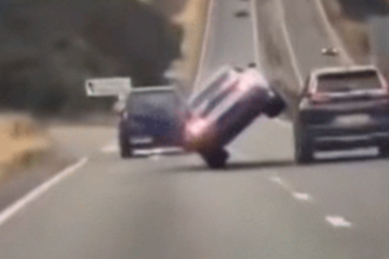
\includegraphics[width=0.40\linewidth]{fig/chap1/ab_start.png}}
      \vspace{0.2cm}
      \subcaptionbox{中速大曲率弯道被动发生 \label{fig:passive_start}}
        {
\includegraphics[width=0.40\linewidth]{fig/chap1/passive_start.png}}
      \subcaptionbox{高速小曲率弯道被动发生 \label{fig:high_start}}  
        {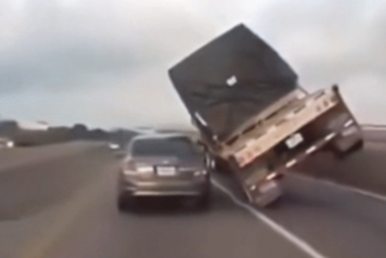
\includegraphics[width=0.40\linewidth]{fig/chap1/high_start.png}}
      \caption{半侧翻态发生的情况}
      \label{fig:semi_rollover_condition}
    \end{figure}

    其次关注半侧翻模态的可控性，如图~\ref{fig:newb_test}所示，2016年11月3日中国车手韩岳驾驶一台MINI完成侧两轮行驶纽伯格林北环全程\SI{20.83}{km}并打破圈速记录；如图~\ref{fig:auto_test}所示，2022年12月，车手田林文驾驶长安览拓者挑战 “汽车侧两轮往返绕桩用时最短”吉尼斯世界记录成功，绕5桩用时\SI{38.41}{s}；如图~\ref{fig:toy_test}工程师对模型玩具车进行改装，通过小型IMU和主动转向控制实现模型车侧两轮行驶；图~\ref{fig:tank_truck_test}是某影视作品中驾驶员进行液罐车半侧翻态行驶的快照截取。通过上述实例总结来说，半侧翻模态在高速和低速都存在可控的状态子空间，半挂液罐车而言同样存在可控的状态子空间，且存在仅通过前轮转向即可控制的区域。在此区域内，通过控制器可以得到与驾驶员控制相同的可控性结论。

    \begin{figure}
      \centering
      \subcaptionbox{纽博格林北环试验场侧两轮行驶 \label{fig:newb_test}}
        {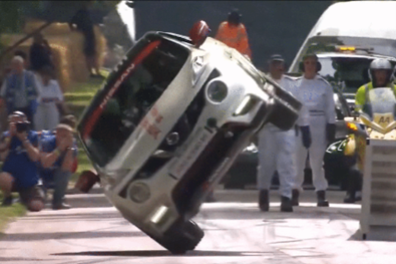
\includegraphics[width=0.40\linewidth]{fig/chap1/newb_test.png}}
      \subcaptionbox{汽车侧两轮往返绕桩挑战现场 \label{fig:auto_test}}
        {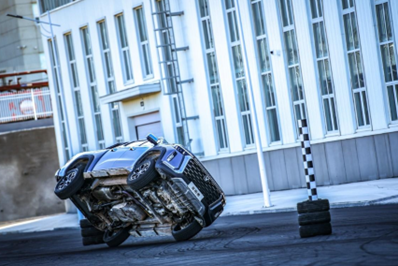
\includegraphics[width=0.40\linewidth]{fig/chap1/auto_test.png}}
      \vspace{0.2cm}
      \subcaptionbox{玩具车靠控制器侧两轮行驶 \label{fig:toy_test}}
        {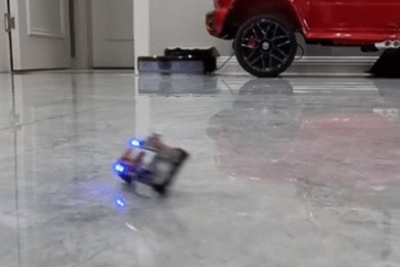
\includegraphics[width=0.40\linewidth]{fig/chap1/toy_test.png}}
      \subcaptionbox{液罐车半侧翻态行驶 \label{fig:tank_truck_test}}  
        {
\includegraphics[width=0.40\linewidth]{fig/chap1/tank_truck_test.png}}
      \caption{半侧翻模态可控性调研}
      \label{fig:semi_rollover_ctrb}
    \end{figure}

  \subsection{强化学习与近端策略优化}  
  \label{sec:rl_overview_ppo}
  强化学习（Reinforcement Learning, RL）研究智能体（agent）在环境（environment）中通过交互学习策略（policy）的过程。典型形式化可用马尔可夫决策过程（Markov Decision Process, MDP）表示：$(\mathcal{S},\mathcal{A},P,r,\gamma)$，其中$\mathcal{S}$为状态空间，$\mathcal{A}$为动作空间，$P(s'|s,a)$为转移概率，$r(s,a)$为即时奖励，$\gamma\in(0,1)$为折扣因子。智能体的目标是最大化期望折扣回报
  \begin{equation}
  J(\pi)=\mathbb{E}_{\tau\sim\pi}\left[\sum_{t=0}^{\infty}\gamma^t r(s_t,a_t)\right],
  \end{equation}
  其中轨迹$\tau=(s_0,a_0,s_1,a_1,\dots)$由策略$\pi(a|s)$诱导。强化学习算法大体可按\emph{值函数学习}、\emph{策略梯度}、\emph{Actor--Critic}与\emph{分布式/改进型}分类，也可以根据是否只用最新策略采集的数据进行训练分为在轨策略（On-Policy）和离轨策略（Off-Policy），其他还有根据策略的随机性与否进行划分的方法等。下文将简述主要RL方法，并简要介绍第\ref{chap03_vehicle_cloud_collaborate}章用到的近端策略优化（Proximal Policy Optimization, PPO）。

  \subsubsection*{(1)基于价值的深度强化学习}
    在离散动作空间中，经典路径是学习动作价值函数$Q^\pi(s,a)$，并通过贪婪策略$ a=\arg\max_a Q(s,a)$做决策。深度Q网络（Deep Q-Network, DQN）将$Q(s,a)$用深度网络近似，并引入经验回放与目标网络稳定训练，是深度强化学习的里程碑工作之一~\cite{DQN_2013}。DQN及后续改进使得在高维观测（如Atari像素）上实现端到端学习成为可能。

    除“期望回报”的标量$Q$，分布式强化学习（Distributional RL）直接建模回报随机变量$Z(s,a)$的分布，并通过分布距离（如Wasserstein/quantile回归）学习更丰富的信息。Bellemare等提出从分布角度刻画强化学习目标，推动了分位数回归DQN等方法的发展~\cite{QR_DQN_2017}。这类思想也可与连续控制的critic建模结合，用于缓解偏差与提升稳定性（如本节的TQC方法）。

  \subsubsection*{(2)策略梯度与Actor--Critic架构}
    当动作空间连续或离散动作规模很大时，直接优化策略$\pi_\bm{\theta}(a|s)$往往更自然。策略梯度方法通过
    \begin{equation}
    \nabla_\bm{\theta} J(\bm{\theta})=\mathbb{E}_{\pi_\bm{\theta}}\left[\nabla_\bm{\theta} \log \pi_\bm{\theta}(a_t|s_t)\, \hat{A}_t \right]
    \end{equation}
    更新参数，其中$\hat{A}_t$为优势函数估计，用于降低方差。异步方法（Asynchronous Methods，通常被称为A3C/A2C范式）通过多线程/多进程并行采样与更新，提高样本效率与训练吞吐~\cite{A2C_2016}。A2C可视为A3C的同步版本，常与广义优势估计（Generalized Advantage Estimation, GAE）等技巧搭配，在中等规模任务中表现相对稳健。

    然而，朴素策略梯度可能因步长过大导致策略崩溃。TRPO通过\emph{信赖域}约束控制新旧策略分布差异（常用KL散度约束），以保证单步更新的“单调改进”倾向~\cite{TRPO_2017}。TRPO理论上优雅，但实现涉及二阶信息与共轭梯度，工程复杂度较高。PPO则用更易实现的“裁剪目标”在一阶优化框架下近似TRPO的保守更新思想~\cite{PPO_2017}，因其鲁棒性与实现简洁成为当前最常用的on-policy基线之一。下一小节将对PPO展开介绍。

  \subsubsection*{(3)连续控制的Off--Policy Actor--Critic架构}
    在连续动作控制中，off-policy Actor--Critic通常更具样本效率。DDPG将确定性策略梯度与Q学习结合，以actor输出连续动作、critic评估$Q(s,a)$，并使用经验回放与目标网络稳定训练~\cite{DDPG_2015}。但DDPG易受函数逼近误差与过估计偏差影响。

    TD3针对DDPG常见问题提出三项关键改进：双Q网络取最小值减少过估计、延迟策略更新降低不稳定、目标策略平滑抑制尖峰~\cite{TD3_2018}。SAC则基于最大熵强化学习框架，在优化期望回报的同时最大化策略熵，从而鼓励探索并提升鲁棒性；其随机策略与温度参数机制使得训练更稳定、性能更强劲~\cite{SAC_2018}。在分布式/分位数视角下，TQC通过\emph{截断}多个分位数critic的尾部来控制过估计偏差，是对连续控制分布式critic的一类有效工程化方案~\cite{TQC_2020}。

  \subsubsection*{(4)其他优化与稳定方法}
    稀疏奖励场景（如机器人到达目标）中，成功轨迹极少导致学习效率低。HER提出“事后经验回放”：将失败轨迹中的达到状态重解释为“目标”，从而为同一条轨迹生成额外的有效监督信号，显著提升样本利用率~\cite{HER_original_2017}。围绕多目标/通用技能学习，Plappert等进一步构建更具挑战的机器人多目标基准与研究议程，推动了多目标强化学习的系统化发展~\cite{plappert2018multigoalreinforcementlearningchallenging}。从工程角度，HER常与DDPG/TD3/SAC等off-policy方法结合，构成解决稀疏奖励连续控制的经典组合。

    除深度Actor--Critic外，参数空间搜索与黑箱优化也能在某些连续控制任务上取得有竞争力的表现。ARS用简单随机方向搜索与归一化技巧，展示了“简单随机搜索”在一些基准上的惊人效果，且实现与调参成本较低~\cite{ARS_2018}。

    近年来，一些工作从\emph{正则化/随机性}或\emph{结构性简化}角度提升样本效率与可扩展性：DroQ通过对Q函数施加dropout并进行多次采样估计，有助于获得更“保守/稳健”的价值估计并提高样本效率~\cite{DroQ_2022}；CrossQ讨论了在深度强化学习中引入（批）归一化以获得更好的样本效率与更简洁的训练配方~\cite{CrossQ_2024}；SimBa则从“simplicity bias”角度讨论参数规模扩展（scaling up）时的训练行为与规律，为大参数RL的可扩展训练提供经验性指引~\cite{SimBa_2025}。这些方向共同反映了一个趋势：在既定算法骨架（如Actor--Critic）上，通过更简单、更稳定的训练配方来获得更强的实际效果。

  \subsubsection*{(5)PPO方法核心思想与目标函数}
    PPO属于\emph{on-policy} Actor--Critic方法，核心目标是在保持实现简单的一阶优化框架下，限制策略更新幅度，避免性能骤降~\cite{PPO_2017}。其关键在于使用重要性采样比率
    \begin{equation}
    r_t(\bm{\theta})=\frac{\pi_\bm{\theta}(a_t|s_t)}{\pi_{\bm{\theta}_{\text{old}}}(a_t|s_t)},
    \end{equation}
    并用优势函数$\hat{A}_t$构建surrogate目标。最常用的PPO-Clip形式为
    \begin{equation}
    L^{\text{CLIP}}(\bm{\theta})=\mathbb{E}_t\left[\min\left(r_t(\bm{\theta})\hat{A}_t,\ \text{clip}(r_t(\bm{\theta}),1-\epsilon_{clip},1+\epsilon_{clip})\hat{A}_t\right)\right],
    \label{eq:ppo_clip}
    \end{equation}
    其中$\epsilon_{clip}$为裁剪阈值（如0.1或0.2）。直观解释如下：
    \begin{itemize}
    \item 当$r_t(\bm{\theta})$偏离1（新旧策略差异过大）且会\emph{过度}提高目标时，裁剪项会限制增益，强制更新更保守。
    \item 通过$\min(\cdot)$结构，PPO在经验上倾向于避免“看似提升但可能导致崩溃”的过大更新。
    \end{itemize}

    PPO还通常加入价值函数损失与熵正则项构成整体目标：
    \begin{equation}
    L(\bm{\theta})=L^{\text{CLIP}}(\bm{\theta})-c_v\,\mathbb{E}_t\left[(V_\bm{\theta}(s_t)-\hat{V}_t)^2\right]+c_e\,\mathbb{E}_t\left[\mathcal{H}(\pi_\bm{\theta}(\cdot|s_t))\right],
    \label{eq:ppo_total}
    \end{equation}
    其中$V_\bm{\theta}$为critic，$\hat{V}_t$为回报/TD目标，$\mathcal{H}$为策略熵，$c_v,c_e$为权重。熵项鼓励探索、降低过早收敛风险；价值损失为actor提供低方差优势估计支撑。PPO的工程实现通常采用“采样一批on-policy轨迹 $\rightarrow$ 多个epoch、小批量SGD更新”的训练范式。

  \subsubsection*{(6)优势函数估计与训练流程}
    PPO性能高度依赖优势函数$\hat{A}_t$的估计质量。常见做法是采用GAE思想构造指数加权的TD残差累积（这里给出常用形式，便于在实现中对齐）：
    \begin{align}
    \delta_t &= r_t + \gamma V(s_{t+1})-V(s_t),\\
    \hat{A}_t &= \sum_{l=0}^{T-t-1}(\gamma\lambda)^l \delta_{t+l},
    \end{align}
    其中$\lambda\in[0,1]$控制偏差--方差权衡。实践中通常对优势做标准化（减均值除标准差），以提升数值稳定性。PPO典型训练步骤可概括为：
    \begin{enumerate}
    \item 使用当前策略$\pi_{\bm{\theta}_{\text{old}}}$在环境中采样$N$步或若干条轨迹，得到$\{(s_t,a_t,r_t,s_{t+1})\}$；
    \item 用critic计算$V(s_t)$并构造$\hat{A}_t$与价值目标$\hat{V}_t$；
    \item 固定旧策略$\pi_{\bm{\theta}_{\text{old}}}$，以小批量方式对目标$L(\bm{\theta})$进行$K$个epoch的梯度更新；
    \item 更新$\bm{\theta}_{\text{old}}\leftarrow \bm{\theta}$，进入下一轮采样。
    \end{enumerate}
    与off-policy方法（DDPG/TD3/SAC）相比，PPO的采样数据必须较新（on-policy），因此样本效率略逊，但其训练稳定性、对超参数的鲁棒性以及在复杂策略网络（如CNN/Transformer）上的泛化表现，使其在很多工程场景依然是首选基线~\cite{PPO_2017}。

\section{理论补充}


  \subsection{图结构与图神经网络}

    \subsubsection*{(1)图数据结构}
      语音、图像、文本等常见结构化数据一般表示为顺序结构，如序列或矩阵，但对更为一般的非结构化数据如知识图谱、社交网络、分子结构等难形成以有效表征。图是一种更为通用的数据结构，能够有效表示实体及其关系。在图中，实体通常表示为节点，而实体之间的关系表示为边，图可以是有向或无向的，节点和边都可以具有一系列如强度、重要性和其他更多维度的特征。图数据结构广泛应用于各种领域，如社交网络分析、推荐系统、生物信息学等，如图~\ref{fig:graph_structure}所示。

      \begin{figure}
        \centering
        \subcaptionbox{知识图谱 \label{fig:knowledge_graph}}
          {
\includegraphics[width=0.3\linewidth]{fig/chap3/knowledge_graph.png}}
        \subcaptionbox{分子结构 \label{fig:moleculer}}
          {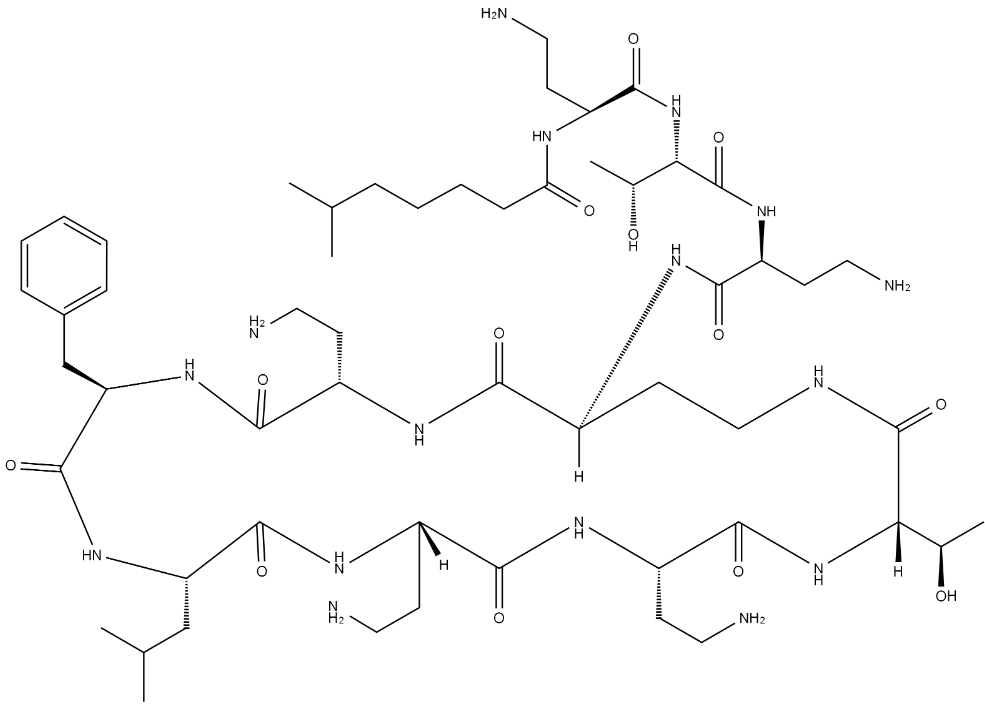
\includegraphics[width=0.3\linewidth]{fig/chap3/moleculer.png}}
        \subcaptionbox{复杂系统 \label{fig:complex_system}}
          {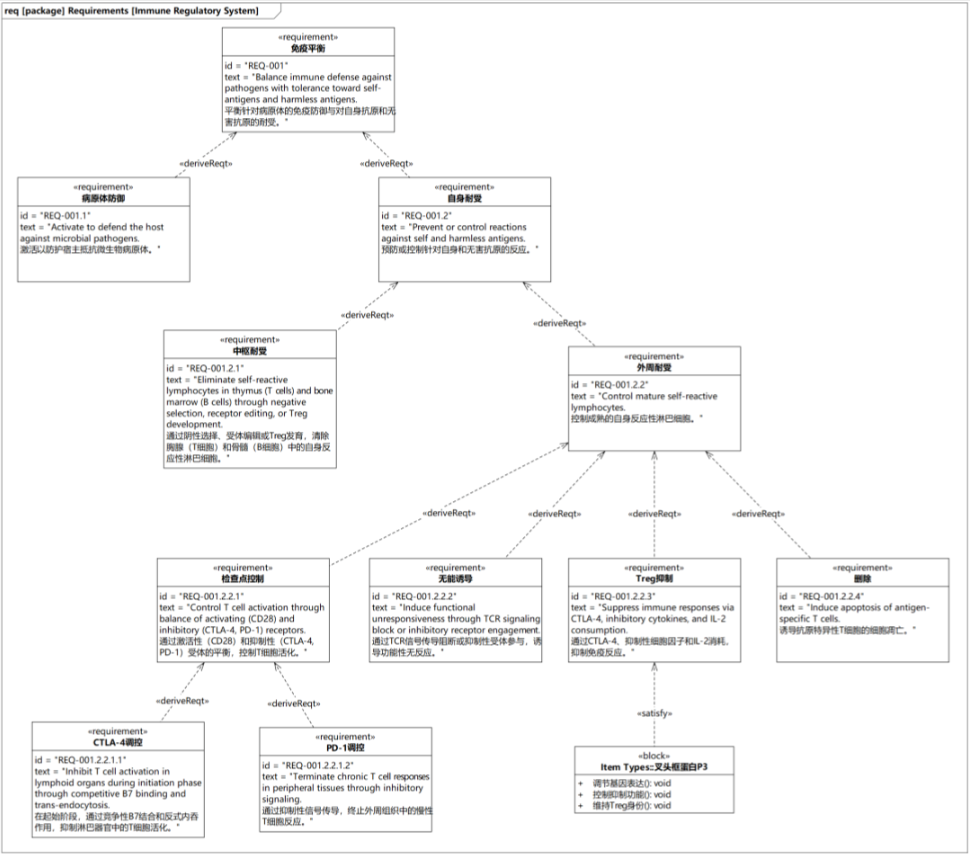
\includegraphics[width=0.26\linewidth]{fig/chap3/complex_system.png}}
        \vspace{0.2cm}
        \subcaptionbox{社交网络 \label{fig:social_network}}
          {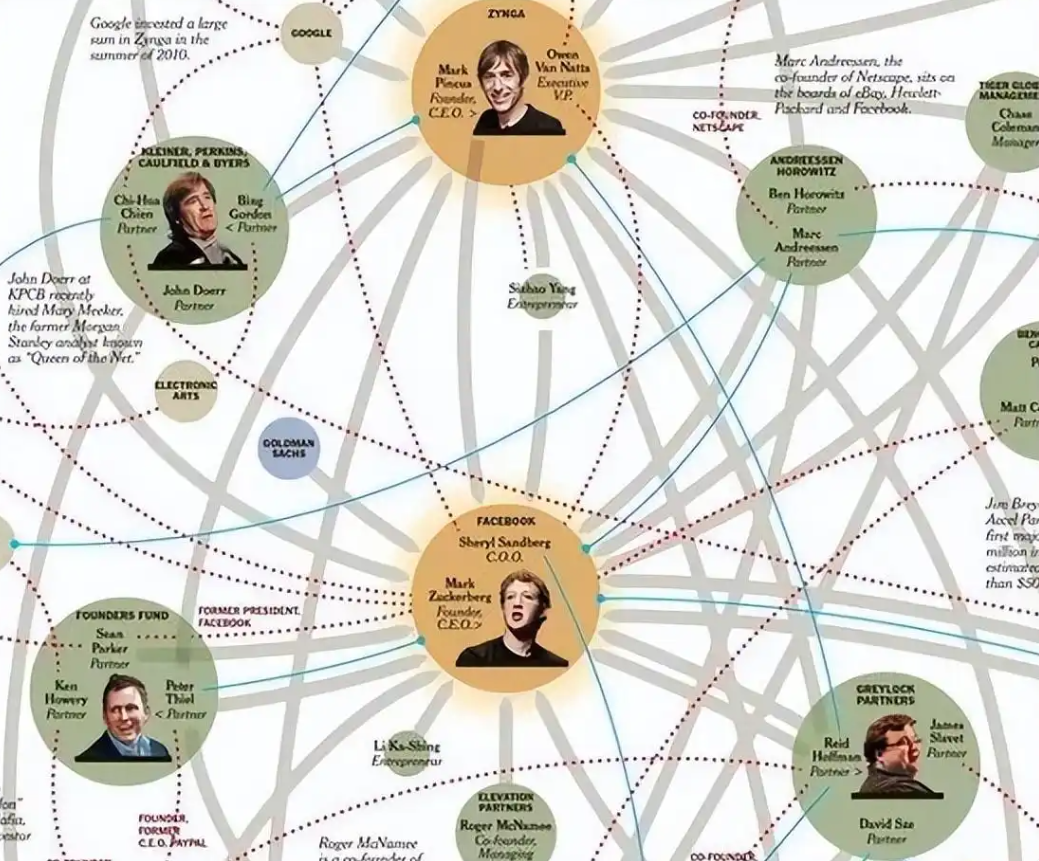
\includegraphics[width=0.3\linewidth]{fig/chap3/social_network.png}}
        \subcaptionbox{交通网络 \label{fig:traffic_net}}  
          {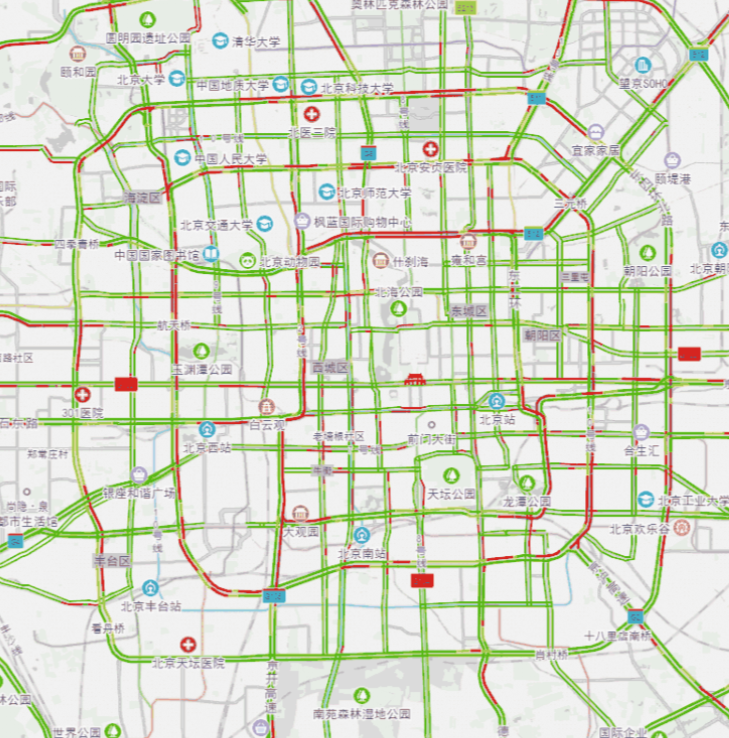
\includegraphics[width=0.25\linewidth]{fig/chap3/traffic_net.png}}
        \subcaptionbox{生物网络 \label{fig:biological_network}}  
          {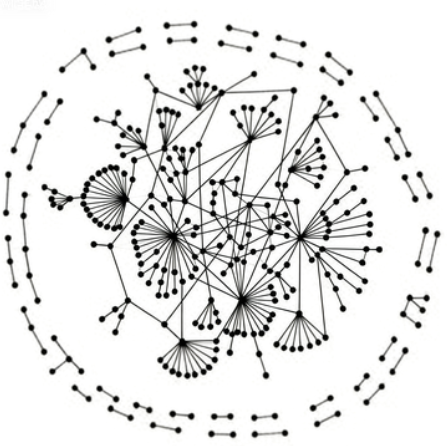
\includegraphics[width=0.27\linewidth]{fig/chap3/biological_network.png}}

        \caption{图结构示例}
        \label{fig:graph_structure}
      \end{figure}

      图结构数据通常具有无序性、异质性、稀疏性等特征。和点云类似，对于图而言节点和边都没有固定的顺序，这种特性称为无序性；图的节点与边的特征通常以向量密集表示为节点特征矩阵$\mathcal{V} \in \mathbb{R}^{n_\mathrm{v} \times d_\mathrm{v}}$和边特征矩阵$\mathcal{E} \in \mathbb{R}^{n_\mathrm{e} \times d_\mathrm{e}}$，其中$n_\mathrm{v}$表示图中节点的数量，$n_\mathrm{e}$表示图中边的数量，$d_\mathrm{v}$表示图中节点的特征维度，$d_\mathrm{e}$表示图中边的特征维度。若一张图中同时存在多种不同维度特征的节点或边，则称该图是异质的。在表达形式上，图$\mathcal{G}$的连接关系通常可以由邻接矩阵$\mathcal{A} \in \mathbb{R}^{n_\mathrm{v} \times n_\mathrm{v}}$表示，元素$a_{ij} \in \left(0, 1\right)$表示节点$\mathrm{v}_i$与节点$\mathrm{v}_j$之间的单向连接关系，故对于无向图而言，邻接矩阵是对称的，而由于连接数通常与节点数量量级类似，故这种连接通常是稀疏的，邻接矩阵$\mathcal{A}$几乎总是可以表征为稀疏形式存储。

      在交通场景中，图可以用于表示道路网络，其中节点表示交叉口或路段甚至道路上的传感器，边表示道路或传感器的连接关系甚至只表示相对位置来体现权重\cite{STGCN2018}。此外，在单车视角的交通预测中，图还可以用于表示交通参与者之间的交互关系，如车辆之间的距离、速度差异等\cite{Wayformer2022}。本质上如文本和图像等顺序结构其实也可以表示为图的特例\cite{VisionGNN2022}。和顺序结构相比，图在提高表达能力的同时也带来了更高的计算复杂度和挑战性，如图的无序性、异构性、稀疏性等问题需要特殊的处理方法。

    \subsubsection*{(2)图神经网络与交通预测}
      图神经网络（Graph Neural Network, GNN）是专为图结构数据而设计的深度学习模型，与全连接网络相比增加了对于邻接矩阵$\mathcal{A}$甚至边特征矩阵$\mathcal{E}$的处理以够有效捕捉带有拓扑结构的图中节点之间、节点与边、边与边的关系。最早的图神经网络是由Kipf和Welling在2016年\cite{GCN2017original}将卷积的概念引入图结构，提出图卷积网络（Graph Convolution Network, GCN）用于图结构数据的局部特征聚合。此后，GNN的研究不断发展，在基础结构上涌现出了许多不同的模型，如在特征聚合上GraphSAGE\cite{GraphSAGE2017}通过采样的方式选取邻居解决大图计算复杂度问题；GAT\cite{GAT2018original}及其改进版GATv2\cite{GATv2_2022}将注意力机制第一次引入邻居聚合中，而HAN\cite{HAN2019}则将局部图注意力进一步推广到了异质图。图结构处理上Cluster-GCN\cite{Cluster_GCN}通过拆分子图实现大图分批计算；SAGPooling\cite{SAGPooling2019}则通过原位降/上采样的方式实现了图池化（Graph Pooling, GPool）的操作，使得多尺度的图操作成为可能，如实现U-Net\cite{U_net2015original}等包含GPool的操作。
      
      上述GNN也称为消息传递网络（Message Passing Network, MPN），实现了沿（有向）边的邻居节点特征聚合。但MPN存在过平滑的问题，表达能力受1-WL测试上限，网络深度普遍无法超过3层，这意味着每个节点最多只能聚合其3阶邻居的特征，无法有效捕捉长距离依赖。基于谱图卷积理论的Chebyshev多项式近似图卷积（ChebConv）被提出以同时聚合$k$阶邻居特征，但仍存在过平滑问题。为进一步提高模型表达能力，让每个节点对全局所有而非仅其邻居节点进行注意力运算特征聚合，图Transformer（Graph Transformer, GT）类模型被提出，如Graphormer\cite{Graphormer2021}引入节点间最短距离矩阵和节点中心性特征等方法编码图结构，并采用标准Transformer进行计算实现了全局图聚合，但未能避免稠密注意力计算量随节点数二次方增长的性能瓶颈；GraphGPS采用位置（Positional Embedding, PE）/结构编码（Structual Embedding, SE）的方式编码局部、全局、相对三类图关系，并利用MPN实现局部消息传递，再利用Performer\cite{Performer2022}或Q-Former\cite{BLIP_2_Q_Former2023}的线性全局注意力全局聚合进一步降低计算复杂度；但PE或SE的计算通常需要较高花费，如随机游走预训练等方式，且对跨图泛化不友好。为进一步提高GT表达能力和更强的跨图泛化性能，Polynomer\cite{Polynomer2024}通过级联全局线性多项式注意力与MPN实现强表达性的同时则省去了PE或SE，直接利用无编码全局注意力运算的置换不变性解决图的无序性问题，将跨图泛化能力推向极致；针对数百万节点级别的超大图，SGFormer则采用单层全局图注意力搭配MPN，虽牺牲了跨图泛化能力，但在大图任务上的效果得到维持。

      GNN在交通预测领域被广泛使用。路网交通预测最早通过图像处理的思路解决，但路网的稀疏性使得视野中绝大部分的非路面区域对预测效果形成严重干扰并提高了计算量。从STGCN\cite{STGCN2018}开始首次将GNN用于交通预测，其将时序卷积网络（Temporal Convolution Network, TCN）与ChebConv结合实现了对交通流量的时空预测；DCRNN\cite{DCRNN2018}则通过引入扩散卷积（Diffusion Convolution, DC）实现了对交通网络中节点间非对称关系的建模，并结合循环神经网络（Recurrent Neural Network, RNN）实现了对交通状态的时序预测；Graph WaveNet\cite{GraphWaveNet2019}通过引入自适应邻接矩阵学习交通网络中节点间动态关系，并结合堆叠扩张因果时序卷积实现了对交通状态的长时域预测；Graph-UNet\cite{U_net_TrafficPred2022}将。近年来，随着GT的发展，基于其的交通预测模型也逐渐兴起。如ASTGNN\cite{ASTGCN2019}通过引入空间和时间注意力机制实现了对交通状态的时空建模；GMAN\cite{GMAN2019}则通过引入门控机制和多头注意力机制提升了交通预测性能；STTN\cite{STTN2021}通过堆叠时空Transformer实现了对交通状态的长时域预测；ST-Mamba\cite{ST_Mamba2024}和SpoT-Mamba\cite{SpoT_Mamba2024}则将基于状态空间模型的Mamba-2\cite{Mamba2_2024}架构引入替代Transformer实现了中小图上更好的效果；BigST\cite{BigST2024}则进一步提高了。这些基于GNN的交通预测模型在处理复杂的交通网络结构和捕捉时空依赖关系方面表现出色，显著提升了交通预测的准确性和鲁棒性。
      
      在云端进行的长时域规划需要面对信息往返传输时延的挑战，且在云控基础平台已经可以直接拿到结构化感知数据，故从计算效率与可实现性角度看，直接以结构化感知数据为输入的决策规划方法更适合在云端进行运行与部署。相比于如基于BEV等感知结构输入的方式\cite{li2024bev_planner}，以图结构进行交通场景感知结果的输入方法为云端长时域非确定性交通预测提供了有效的技术手段。

  \subsection{流匹配扩散方法}
      流匹配（Flow Matching, FM）是一种基于向量流场理论的生成模型，用于学习数据分布的速度向量场。其核心思想是通过最小化数据样本与模型生成样本之间的流匹配损失，来训练一个能够生成目标分布样本的模型\cite{FlowMatching2023original}。相比于DDPM等基于扩散模型的生成方法，FM无需显式定义扩散过程，直接学习数据分布的速度向量场，在样本生成上有显著效率，甚至可以一步生成高质量样本\cite{GoalFlow2025}。

      在图像生成中，每个像素点的RGB值代表3维度向量，像素点数为$N_{pix}$，则可以看成在$3 N_{pix}$维向量空间中进行流匹配；在轨迹生成上，如果以\SI{10}{Hz}生成未来\SI{8}{s}的包含$x,y$的轨迹，则相当于在160维向量空间进行流匹配。

      FM用神经网络学习一个任务向量空间上的向量流场：$v_t^\bm{\theta}$，其损失函数定义为
      \begin{equation}
      \mathcal{L}(\bm{\theta}) = \mathbb{E_{t,p_t(x)}} \lVert v_t^\bm{\theta}(x_t) - v_t^{target}(x_t) \rVert^2
      \label{eq:fm_loss_original}
      \end{equation}

      其中$\bm{\theta}$表示神经网络的参数，$t \in [0,1]$表示时间变量，$x_t$表示在时间$t$时刻的样本，$p_t(x)$表示在时间$t$时刻的样本分布，$v_t^{target}(x_t)$表示在时间$t$时刻的目标速度向量场。
      
      为获得$v_t^{target}(x_t)$，在生成式FM任务中通常需自行构建一个流。我们首先构造一个从原始分布$p_0(x)$到目标分布$p_1(x)$的平滑过渡连续分布族$p_t(x)$，$t\in [0,1]$，$p_t(x)$平滑地从$p_0(x)$过渡到$p_1(x)$:

      \begin{equation}\psi_t^{target}(x_0|z)=\alpha_t z+ \beta_t x_0 
      \end{equation}

      其中$x_0 \sim p_0(x)$是采样自已知初始分布的样本，$z \sim p_1(x)$是采样自真实分布的样本。最常用的是衍生自最优传输理论且最简单直观的整合流（Rectified Flow）,即对原始分布和目标分布进行线性插值，定义如下：

      \begin{equation} \psi_t^{target}(x_0|z) = x_t = t z + (1-t)x_0 
      \end{equation}

      除了线性插值，也可用指数插值$x_t = e^{-t}x_0 + (1-e^{-t})z$，核心是保证$p_t(x)$的连续性。则速度向量场的目标为：

      \begin{equation} v_t^{target}(x_t|z) = v_t^{target}(\psi_t^{target}(x_0|z)|z) \\
      = \frac{\mathrm{d}\psi_t^{target}(x_0|z)}{\mathrm{d}t} = \frac{\mathrm{d}\alpha_t}{\mathrm{d}t} z + \frac{\mathrm{d}\beta_t}{\mathrm{d}t} x_0
      \end{equation}

      其中$\alpha_t$和$\beta_t$分别表示时刻$t$对目标样本和已知初始样本的线性插值系数。对整合流而言，条件目标速度向量场为：

      \begin{equation} v_t^{target}(x_t|z) = z - x_0 \end{equation}

  \subsection{图扩散流匹配理论证明}
  \label{sub:graphflow_proof}
    我们希望学习得到的是动态特征速度的边缘向量场：$v_t^\bm{\theta}$，其不依赖于未来真值$\mathcal{V}_{k+1}$，那么我们使用条件向量场计算出来的速度向量$v_t^{target}(F_{dyn}^{t}|\mathcal{V}_{k+1})$是否可以拿来当做训练的标签，即是否可以将无条件损失式\eqref{loss_fm}替换为有条件损失式\eqref{loss_cfm}。

    \begin{equation}\mathcal{L}_{FM}(\bm{\theta}) = \mathbb{E_{t\sim\mathcal{U},x\sim p_t}} \left[\lVert v_t^\bm{\theta}(F_{dyn}^{t}) - v_t^{target}(F_{dyn}^{t}) \rVert^2 \right]\label{loss_fm}\end{equation}

    \begin{equation}\mathcal{L}_{CFM}(\bm{\theta}) = \mathbb{E_{t\sim\mathcal{U},x\sim p_t(\cdot|z),z\sim p_1}} \left[\lVert v_t^\bm{\theta}(F_{dyn}^{t}) - v_t^{target}(F_{dyn}^{t}|\mathcal{V}_{k+1}) \rVert^2 \right]\label{loss_cfm}\end{equation}

    其实是可以的，下面来进行证明：

    为了简化证明过程，不妨令真值$z = \mathcal{V}_{k+1}$，动态特征场$x = F_{dyn}^{t}$。我们有了条件向量场，现在需要求出边缘向量场，也就是不依赖于$z$的向量场。边缘概率路径是对条件概率路径乘以条件$z$的概率然后对所有可能的$z$积分，即
    \begin{equation}p_t(x) = \int_{z} p_t(x|z)p_1(z)\mathrm{d}z\end{equation}
    本质上应用了全概率公式，按照各种条件对$z$进行汇总，然后对所有可能的$z$积分。那么是否可以通过对所有条件向量场乘以$p(z)$，然后对所有可能的$z$积分，得到边缘向量场？即
    \begin{equation}v_t^{target}(x) = \int_{z} v_t^{target}(x|z)p_1(z)\mathrm{d}z\end{equation}

    答案是不行的，因为这里的$v_t^{target}$是个向量场，不是概率值，不能应用全概率公式。实际上的公式是这样的

    \begin{equation}v_t^{target}(x) = \int_{z} v_t^{target}(x|z)p_t(z|x)\mathrm{d}z\end{equation}

    我们可以利用贝叶斯公式$p_t(z|x)=\frac{p_t(x|z)p(z)}{p_t(x)}$转化一下上述边缘向量场公式，得到
    \begin{equation}v_t^{target}(x) = \int_{z} v_t^{target}(x|z)\frac{p_t(x|z)p_1(z)}{p_t(x)}\mathrm{d}z\end{equation}
    这个表达式在后面证明时会用到。

    接下来就来证明为什么边缘向量场的公式是那样的。我们需要验证的是这个边缘向量场公式符合连续性方程：

    \begin{equation}\frac{\partial p_t(x)}{\partial t} + \nabla \left(p_t(x) v_t^{target}(x)\right) =0\end{equation}

    \begin{proof}
      \begin{theorem}[连续性方程]
        设存在流，其质量场为$\rho$，速度场为$\mathbf{v}$，时间变量为$t$，则流场满足：
        \begin{equation}
          \frac{\partial \rho}{\partial t} + \nabla \cdot (\rho \mathbf{v}) = 0
        \end{equation}
      \end{theorem}
      连续性方程第一项，概率密度对时间求导，代入边缘概率的公式
      \begin{equation}\frac{\partial p_t(x)}{\partial t} = \frac{\partial}{\partial t}\int_z p_t(x|z)p_1(z)\mathrm{d}z\end{equation}
      然后将求导符号移入积分符号，其中$p(z)$可以看做常数项
      \begin{equation}= \int_z \frac{\partial p_t(x|z)}{\partial t}p_1(z)\mathrm{d}z\end{equation}
      偏导部分满足连续方程，可代入
      \begin{equation}= \int_z -\nabla \left(p_t(x|z) v_t^{target}(x|z)\right)p_1(z)\mathrm{d}z\end{equation}
      因为散度计算是对$x$进行的，而这里的积分是对$z$进行的，所以可以将散度符号移到积分号外边
      \begin{equation}= -\nabla \left(\int_z p_t(x|z) v_t^{target}(x|z)p_1(z)\mathrm{d}z\right)\end{equation}
      下一步在积分号外乘$p_t(x)$，在积分号内除$p_t(x)$，得到
      \begin{equation}= -\nabla \left(p_t(x)\int_z  v_t^{target}(x|z)\frac{p_t(x|z)p_1(z)}{p_t(x)}\mathrm{d}z\right)\end{equation}
      可以发现这里的积分项就是我们之前定义的边缘向量场公式，故上式为
      \begin{equation} = -\nabla \left(p_t(x) v_t^{target}(x)\right)\end{equation}
      证明完毕。
  \end{proof}
  故上述流匹配过程在未来预测上应满足连续性方程，从而保证了通过条件流匹配学习得到的边缘向量场的正确性。同时，可以保证自车和周车存在概率在宏观扩散过程中保持一致，即使原本集中的概率扩散到更宽阔的道路空间中以更低的概率存在。

  \subsection{面向半挂车的修正紧急因子指标推导计算}
  \label{sub:trailer_mei_proof}
    目前一维替代安全指标（Surrogate Safty Index, SSI）如碰撞时间（Time to Collision, TTC）、车头时距（Time Head Way, THW）等仅在跟车情况下有效，不考虑车辆真实宽度与几何形状，对二维空间中的碰撞无法有效监测；而二维碰撞指标如RTTC虽考虑二维几何形状，对斜碰等问题可以探测，但计算过于乐观且不考虑不同撞击重叠面积风险的不同。Cheng等震碎上述问题在2024年提出紧急因子（Emergency Index, EI）\cite{chenghao2025emergency_index}安全评价指标，并在2025年进一步提出修正紧急因子（Modified Emergency Index, MEI）\cite{chenhao2025mei}。

    MEI通过计算侵入距离（InDepth）来评估车辆最大的安全损失，计算紧急操作时间（Time for Emergency Maneouvour, TEM）即可用于规避风险的操作时间来衡量风险的紧急程度，其定义为：
    \begin{equation}
      \text{MEI} = \frac{\text{InDepth}}{\text{TEM}}
    \end{equation}
    其中InDepth如图~\ref{fig:indepth}所示，定义为自车和周车都匀速直线运动的前提假设下，将周车在未来无限时域内的空间位置投影在自车坐标系下以后，自车轮廓与周车投影相交的最大距离。当沿着匀速直线运动可能发生碰撞时，InDepth大于0，否则InDepth小于0。
    \begin{figure}
      \centering
      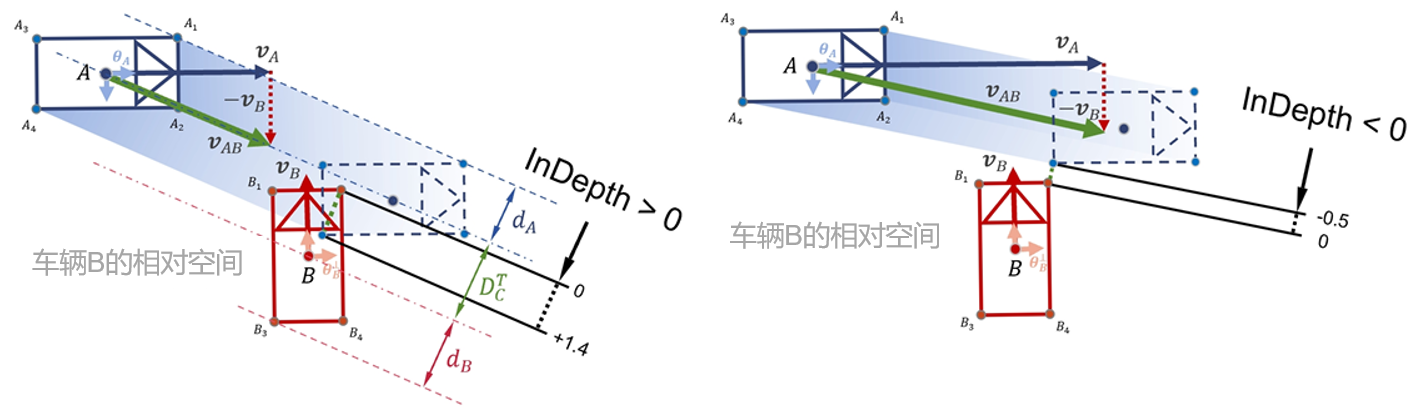
\includegraphics[width=1.0\linewidth]{fig/appx/indepth_illust.png}
      \caption{InDepth概念描述}
      \label{fig:indepth}
    \end{figure}
    TEM定义为自车和周车都匀速直线运动的前提假设下，两车轮廓最早发生重叠的时间，若不发生重叠则$\text{TEM} = \infty$。

    MEI经过对比测试，相比于现有二维SSI能够有效反映车辆实际风险，且计算速度很快，经过C++编译后单次计算时间大约在\SIrange{6}{10}{\micro s}。但MEI仍存在一些问题，如其匀速直线运动假设过强，且针对如环岛等匀速恒定前轮转角的情况适用性较差，以及针对本文而言，其无法计算辆车中其一或全部为半挂车时的风险，即只能针对两辆单车计算风险。为对包含挂车的车辆对（Vehicle Pair）计算MEI指标，本文提出面向半挂车的修正紧急因子（trailer-oriented modified emergency index, Trailer-MEI）方法。

    假设半挂车的牵引车部分匀速直线运动，挂车后轴轨迹为曳物线（tractix），如图~\ref{fig:drag_line}所示，设铰接角为$\gamma_{g}$，牵引车车速为$v_{1x}$，其解析形式可描述为式\eqref{eq:theta}到式\eqref{eq:trailer_traj}。其中铰接角随时间变化为$\gamma_{g}(t)$如式\eqref{eq:theta}所示，则牵引车轨迹直线为式\eqref{eq:tractor_traj}，挂车曳物线为式\eqref{eq:trailer_traj}。

    \begin{figure}
      \centering
      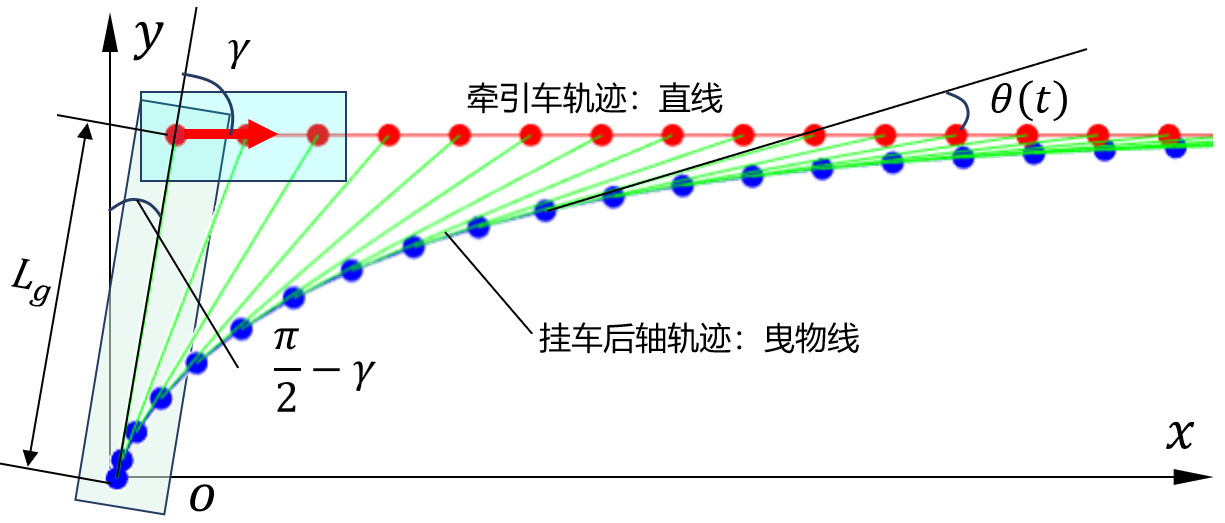
\includegraphics[width=0.7\linewidth]{fig/appx/drag_line.png}
      \caption{挂车曳物线轨迹}
      \label{fig:drag_line}
    \end{figure}

    \begin{equation}
      \gamma_{g}(t) = \pi - 2 \arctan\left( \tan\frac{\pi - \gamma_{g}}{2}  e^{\frac{v_{1x}}{L_g} t} \right)
      \label{eq:theta}
    \end{equation}
    \begin{equation}
      x_{\text{tractor}}(t) = v_{1x}   t + L_g   \cos\gamma_{g},
      \quad
      y_{\text{tractor}}(t) = L_g   \sin\gamma_{g}
      \label{eq:tractor_traj}
    \end{equation}
    \begin{equation}
      \begin{aligned}
      x_{\text{trailer}}(t) &= - L_g  \left( \ln\left( \tan\frac{\gamma_{g}(t)}{2} + \cos\gamma_{g}(t) \right) \right) + L_g  \left( \ln\left( \tan\frac{\gamma_{g}}{2} + \cos\gamma_{g} \right) \right) 
      \\
      y_{\text{trailer}}(t) &= -L_g   \left( \sin\gamma_{g}(t) - \sin\gamma_{g} \right)
      \end{aligned}
      \label{eq:trailer_traj}
    \end{equation}

    由于将曳物线根据相对自车车速投影到坐标系后并没有和直线相交的解析解存在，故需采用数值方法进行近似。为计算在曳物线上距离均匀划分的采样点，如图~\ref{fig:trailer_proj}所示，采用对时间$t$进行均匀划分的方法，得到$N_{pred}$个时间点$t_1, t_2, \dots, t_{N_{pred}}$对应的角度$\gamma_{g}(t)$，从而可以计算出$N_{pred}$个挂车轮廓位置$B_g^k,k\in\{1,2,\cdots,N_{pred}\}$。可包含半挂车的车辆对共有三种情况：全无挂车、其一有挂车、两者都有挂车。对于第一种情况可以直接采用MEI进行计算；对第二种情形，假设A车为半挂车B车为单车，需要计算A车牵引车与B车的MEI，以及利用离散的时间分别将平移后的A车挂车轮廓$B_g^{k,\prime}$与B车车头轮廓$B_{veh}$进行$N_{pred}$次碰撞检测与InDepth计算，InDepth解析计算方法见\cite{chenhao2025mei}，假设$t_k$时刻挂车发生碰撞，则挂车与自车计算的等效MEI指标为$\tilde{\text{MEI}}=\frac{\text{InDepth}}{t_k}$，最终取$\text{Trailer-MEI} = \max(\tilde{\text{MEI}},\text{MEI})$；对于第三种情况，需要验证A车与B车车头的MEI，以及A车车头与B车挂车、B车车头与A车挂车在第二种情况的$\tilde{\text{MEI}}_1$和$\tilde{\text{MEI}}_2$，并分别对两车挂车在$N_{pred}$个时刻的绝对轮廓进行InDepth计算，计算过程不再赘述，最终取4者中最大者为此情况的Trailer-MEI。

    \begin{figure}
      \centering
      \subcaptionbox{挂车曳物线轨迹投影 \label{fig:trailer_proj}}
        {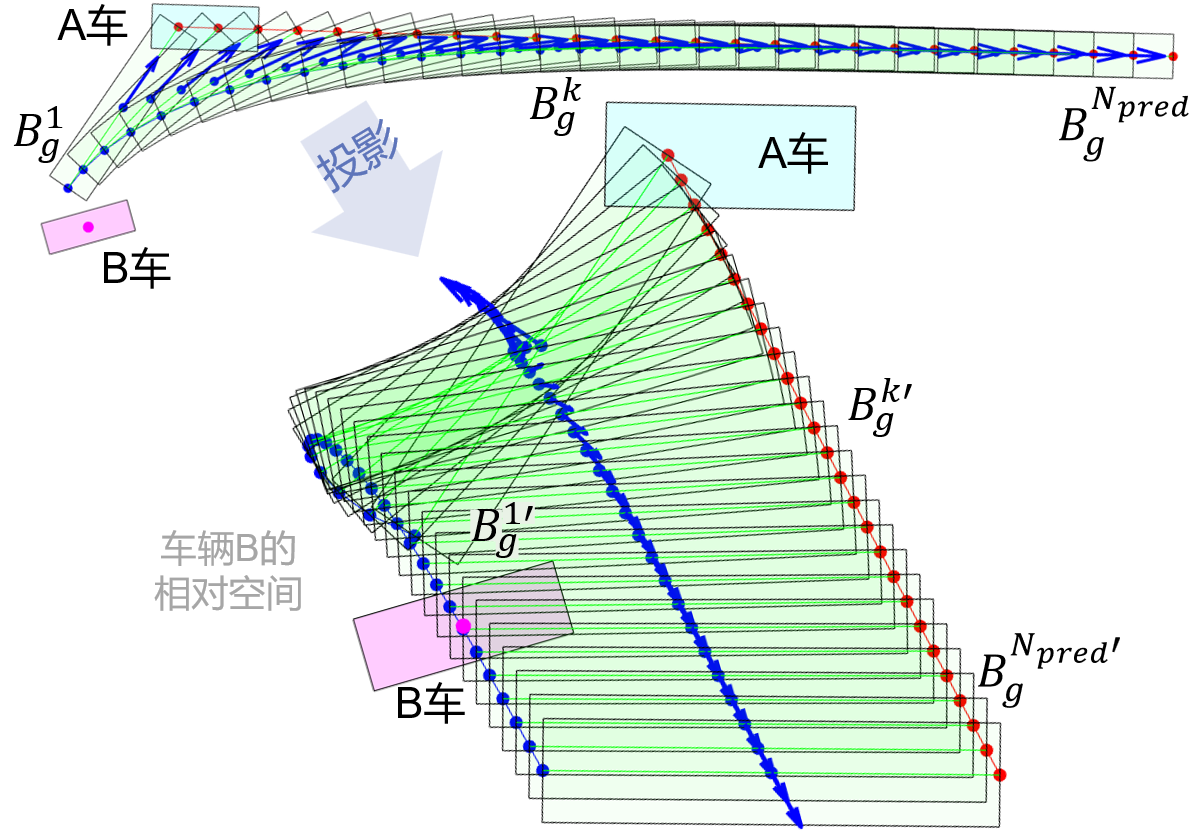
\includegraphics[width=0.5\linewidth]{fig/appx/trailer_proj.png}}
      \subcaptionbox{挂车与挂车间计算 \label{fig:trailer_calc}}
        {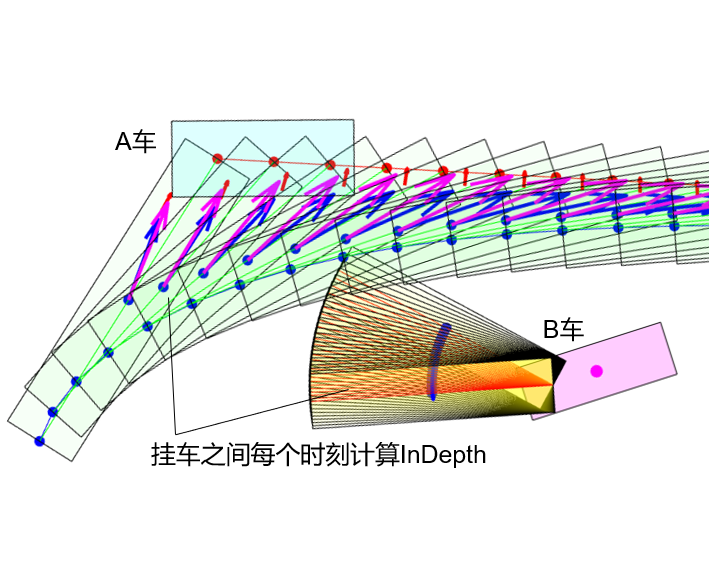
\includegraphics[width=0.48\linewidth]{fig/appx/trailer_calc.png}}

      \caption{包含挂车的计算示意}
      \label{fig:trailer_proj_calc}
    \end{figure}

    在最坏情况，即需计算SSI的辆车都为半挂车时，Trailer-MEI指标的计算时间仅为MEI的6倍，C++编译后单次计算时间大约在\SIrange{30}{50}{\micro s}，在实现半挂车间计算的同时计算时间依然可以忽略。本文为平衡精度与计算速度，计算Trailer-MEI指标采用的离散步长$\increment t = \SI{0.2}{s}$，预测时域为\SI{5}{s}。



  \subsection{无模型自适应滑模残差补偿}
    \label{sub:MFASMC_residual_compensation}

    第\ref{sub:multi_constraint_mpc}小节构建的多约束模型预测控制基础控制器的基本要求在于预测模型的准确性，而这一点在实际行驶过程中由于载荷变化、零部件老化、标定测量误差等原因通常难以绝对保障，对基础模型进行补偿是模型预测方法跨入真正实用的重要部分\cite{tangzeyue2023mpcmfac}。本小节在基础控制器上进一步建立基于广义跟踪误差控制车轮转角和/或各车轮驱/制动力的补偿控制器。广义跟踪误差为牵引车实际轨迹与最优控制下的预测轨迹之间的误差；补偿控制器为无模型自适应滑模控制器，以广义跟踪误差为输入量$\boldsymbol{y}$，并采用全格式动态线性化。下面进行详细说明。

    \begin{figure}
    \centering
    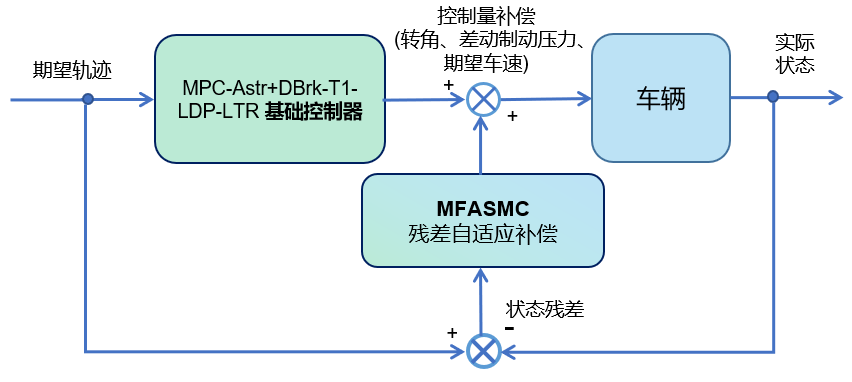
\includegraphics[width=0.8\linewidth]{fig/chap4/mfasmc_sup.png}
    \caption{无模型自适应滑模残差补偿控制器结构}
    \label{fig:mfasmc_sup}
    \end{figure}

    定义 MIMO 非线性系统如下
    \begin{equation}
    \boldsymbol{y}(k + 1) = \boldsymbol{f}\left(\boldsymbol{y}(k), \dots, \boldsymbol{y}(k - n_y), \boldsymbol{u}(k), \dots, \boldsymbol{u}(k - n_u)\right)
    \label{eq:mimo_nonlinear}
    \end{equation}
    式中$\boldsymbol{f}(\cdot)$为未知的非线性函数，$n_y$和$n_u$分别为系统控制和输入的真实阶数，$\boldsymbol{y}(k) \in \mathbb{R}^{N_y}$，$\boldsymbol{u}(k) \in \mathbb{R}^{N_u}$分别为$k$时刻的系统输出和输入，$N_u \geq N_y$。
    由于系统的实际阶数可能很高，为简化模型设置两个固定的伪阶数$L_y$和$L_u$($1 \leq L_y \leq n_y$, $1 \leq L_u \leq n_u$)来代表实际阶数，维护一个固定窗口内的信息向量：
    \begin{equation}
    \boldsymbol{H}_{L_y,L_u}(k) = \begin{bmatrix}
    \boldsymbol{y}(k) \\
    \vdots \\
    \boldsymbol{y}(k - L_y + 1) \\
    \boldsymbol{u}(k) \\
    \vdots \\
    \boldsymbol{u}(k - L_u + 1)
    \end{bmatrix} \in \mathbb{R}^{N_y L_y + N_u L_u}
    \label{eq:info_vector}
    \end{equation}

    对于 MIMO 系统，首先需要定义两个前提条件：
    ① 除有限时刻点外，$\boldsymbol{f}(\cdot)$对于控制变量的偏导数连续；（一般非线性控制的典型约束条件）
    ② 广义 Lipschitz 条件：对任意$k_1 \neq k_2$，$k_1,k_2 \geq 0$，以及$\boldsymbol{H}_{L_y,L_u}(k_1) \neq \boldsymbol{H}_{L_y,L_u}(k_2)$，有
    \begin{equation}
    \|\boldsymbol{y}(k_1 + 1) - \boldsymbol{y}(k_2 + 1)\| \leq b \left\| \boldsymbol{H}_{L_y,L_u}(k_1) - \boldsymbol{H}_{L_y,L_u}(k_2) \right\|
    \label{eq:general_lipschitz}
    \end{equation}
    其中$b > 0$为常数。（信息向量的有限变化不能引起系统输出的无限增长）\cite{houzhongsheng2011book_MFAC}。

    第一个条件是控制系统设计中对一般非线性控制的典型约束，第二个条件是对系统输出变化率上界的一种限制，上述两个条件一般的非线性系统都可以满足。

    给定正整数伪阶数$L_y$和$L_u$，当$\boldsymbol{H}_{L_y,L_u}(k) \neq 0$时，一定存在一个时变的分块伪 Jacobian 矩阵（PPJM）或者叫作伪梯度$\boldsymbol{\Phi}_{f,L_y,L_u}(k)$，使得被控系统能够转化为如下三种数据模型之一（动态线性化模型，Dynamic Linearization, DL）：

    全格式（Full Form DL, FFDL）：包含所有历史信息和高阶动态，建模精度高但伪梯度维度高导致计算量较大，对实时性要求较高的系统可能存在延迟风险，适用于复杂慢时变系统。
    \begin{equation}
    \Delta \boldsymbol{y}(k + 1) = \boldsymbol{\Phi}_{f,L_y,L_u}(k) \Delta \boldsymbol{H}_{L_y,L_u}(k)
    \label{eq:ffdl}
    \end{equation}

    偏格式（Partial Form DL, PFDL）：包含部分历史信息和动态，考虑了系统的记忆特性（如惯性和滞后），计算复杂度适中，可以建模适于中等复杂度系统。
    \begin{equation}
    \boldsymbol{y}(k + 1) = \boldsymbol{y}(k) + \boldsymbol{\Phi}_{p,L_u}(k) \Delta \boldsymbol{H}_{L_u}(k)
    \label{eq:pfdl}
    \end{equation}

    紧格式（Compact Form DL, CFDL）：不包含历史信息，仅将系统输出变化直接与当前输入变化想光临，忽略中间状态变量，形式最为简洁，适用于简单系统。
    \begin{equation}
    \Delta \boldsymbol{y}(k + 1) = \boldsymbol{\phi}(k) \Delta \boldsymbol{u}(k)
    \label{eq:cfdl}
    \end{equation}

    \begin{table}[htbp]
    \small
    \centering
    \caption{三种动态线性化方法对比}
    \begin{tabularx}{\linewidth}{cccccX}
        \toprule
        形式 & 伪梯度维度 & 历史数据依赖 & 精度 & 复杂度 & 适用场景 \\
        \midrule
        紧格式（CF） & 低维向量/标量 & 无/极少 & 低 & 低 & 简单系统实时性要求高 \\
        偏格式（PF） & 中维向量 & 部分历史数据 & 中 & 中 & 中等动态复杂系统 \\
        全格式（FF） & 高维向量 & 全部历史数据 & 高 & 高 & 复杂慢时变系统 \\
        \bottomrule
    \end{tabularx}
    \label{tab:dl_methods_compare}
    \end{table}

    其中
    \begin{equation}
    \Delta \boldsymbol{H}_{L_y,L_u}(k) = \boldsymbol{H}_{L_y,L_u}(k) - \boldsymbol{H}_{L_y,L_u}(k - 1) = \begin{bmatrix}
    \Delta \boldsymbol{y}(k) \\
    \vdots \\
    \Delta \boldsymbol{y}(k - L_y + 1) \\
    \Delta \boldsymbol{u}(k) \\
    \vdots \\
    \Delta \boldsymbol{u}(k - L_u + 1)
    \end{bmatrix}
    \label{eq:delta_H}
    \end{equation}
    \begin{equation}
    \boldsymbol{\Phi}_{f,L_y,L_u}(k)_{N_y \times (N_y L_y + N_u L_u)} = \left[ \boldsymbol{\phi}_1(k)\ \ \cdots\ \ \boldsymbol{\phi}_{L_y}(k)\ \ \boldsymbol{\phi}_{L_y+1}(k)\ \ \cdots\ \ \boldsymbol{\phi}_{L_y+L_u}(k) \right]
    \label{eq:phi_matrix}
    \end{equation}
    其中
    \begin{equation}
    \boldsymbol{\phi}_i(k) = \begin{bmatrix}
    \varphi_{i,11}(k) & \varphi_{i,12}(k) & \cdots & \varphi_{i,1N_y}(k) \\
    \varphi_{i,21}(k) & \varphi_{i,22}(k) & \cdots & \varphi_{i,2N_y}(k) \\
    \vdots & \vdots & \ddots & \vdots \\
    \varphi_{i,N_y 1}(k) & \varphi_{i,N_y 2}(k) & \cdots & \varphi_{i,N_y N_y}(k)
    \end{bmatrix} \in \mathbb{R}^{N_y \times N_y},\ i = 1,\dots,L_y
    \label{eq:phi_i}
    \end{equation}
    \begin{equation}
    \boldsymbol{\phi}_j(k) = \begin{bmatrix}
    \varphi_{j,11}(k) & \varphi_{j,12}(k) & \cdots & \varphi_{j,1N_u}(k) \\
    \varphi_{j,21}(k) & \varphi_{j,22}(k) & \cdots & \varphi_{j,2N_u}(k) \\
    \vdots & \vdots & \ddots & \vdots \\
    \varphi_{j,N_y 1}(k) & \varphi_{j,N_y 2}(k) & \cdots & \varphi_{j,N_y N_u}(k)
    \end{bmatrix} \in \mathbb{R}^{N_y \times N_u},\ j = L_y + 1,\dots,L_y + L_u
    \label{eq:phi_j}
    \end{equation}

    MFAC基础算法与相关符号说明见附录\ref{sub:mfac_basic}小节，本小节在此基础上进一步设计MFASMC控制算法，将 MFAC 与滑模控制结合，前者无需第一性原理模型，后者响应速度快、抗扰动性能强。

    定义输出误差：
    \begin{equation}
    \boldsymbol{e}(k) = \boldsymbol{y}^*(k) - \boldsymbol{y}(k)
    \label{eq:output_error}
    \end{equation}

    设计一个线性滑模面：
    \begin{equation}
    \boldsymbol{s}(k) = \boldsymbol{\Lambda} \boldsymbol{e}(k)
    \label{eq:linear_surface}
    \end{equation}
    其中$\boldsymbol{\Lambda}$是正定矩阵，一般是正定对角阵用于加权各个滑模面。
    \begin{equation}
    \begin{aligned}
    \boldsymbol{s}(k + 1) = \boldsymbol{\Lambda} \boldsymbol{e}(k + 1) = \boldsymbol{\Lambda} \left( \boldsymbol{y}^*(k + 1) - \boldsymbol{y}(k) - \boldsymbol{\Phi}_{f,L_y,L_u}(k) \Delta \boldsymbol{H}_{L_y,L_u}(k) \right) \\
    = \boldsymbol{\Lambda} \left( \boldsymbol{y}^*(k + 1) - \boldsymbol{y}(k) - \sum_{i=1}^{L_y} \boldsymbol{\phi}_i(k) \Delta \boldsymbol{y}(k - i + 1) - \sum_{i=2}^{L_u} \boldsymbol{\phi}_{i+L_y}(k) \Delta \boldsymbol{u}(k - i + 1) \right) - \boldsymbol{\Lambda} \boldsymbol{\phi}_{L_y+1}(k) \Delta \boldsymbol{u}(k)
    \end{aligned}
    \label{eq:surface_next}
    \end{equation}

    设计或选择一个趋近律，比如
    等速趋近律：(其中$\boldsymbol{E} \in \mathbb{S}^{++}$)
    \begin{equation}
    \dot{\boldsymbol{s}} = -\boldsymbol{E} \mathrm{sgn}(\boldsymbol{s})
    \label{eq:reach_law_const}
    \end{equation}
    \begin{equation}
    \boldsymbol{s}(k + 1) = \boldsymbol{s}(k) - T \boldsymbol{E} \mathrm{sgn}(\boldsymbol{s}(k))
    \label{eq:reach_law_const_discrete}
    \end{equation}
    指数趋近律：(其中$\boldsymbol{E} \in \mathbb{S}^{++}, \boldsymbol{K} \in \mathbb{S}^{++}$)
    \begin{equation}
    \dot{\boldsymbol{s}} = -\boldsymbol{E} \mathrm{sgn}(\boldsymbol{s}) - \boldsymbol{K} \boldsymbol{s}
    \label{eq:reach_law_exp}
    \end{equation}
    \begin{equation}
    \boldsymbol{s}(k + 1) = (\boldsymbol{I} - T \boldsymbol{K}) \boldsymbol{s}(k) - T \boldsymbol{E} \mathrm{sgn}(\boldsymbol{s}(k))
    \label{eq:reach_law_exp_discrete}
    \end{equation}
    幂次趋近律：(其中$\boldsymbol{E} \in \mathbb{S}^{++}, \boldsymbol{K} \in \mathbb{S}^{++}, \alpha > 0$)
    \begin{equation}
    \dot{\boldsymbol{s}} = -\left( \boldsymbol{E} + \boldsymbol{K} \mathrm{diag}(|\boldsymbol{s}|^\alpha) \right) \mathrm{sgn}(\boldsymbol{s})
    \label{eq:reach_law_power}
    \end{equation}
    \begin{equation}
    \boldsymbol{s}(k + 1) = \boldsymbol{s}(k) - T \left( \boldsymbol{E} + \boldsymbol{K} \mathrm{diag}(|\boldsymbol{s}(k)|^\alpha) \right) \mathrm{sgn}(\boldsymbol{s}(k))
    \label{eq:reach_law_power_discrete}
    \end{equation}
    这里选取指数趋近律 \eqref{eq:reach_law_exp_discrete} 与 \eqref{eq:surface_next} 联立可以求解出滑模控制意义下的控制量增量
    \begin{equation}
    \Delta \boldsymbol{u}(k) = \boldsymbol{\phi}_{L_y+1}^\dagger(k) \left( \begin{aligned}
    &\boldsymbol{y}^*(k + 1) - \boldsymbol{y}(k) - \sum_{i=1}^{L_y} \boldsymbol{\phi}_i(k) \Delta \boldsymbol{y}(k - i + 1) - \sum_{i=2}^{L_u} \boldsymbol{\phi}_{i+L_y}(k) \Delta \boldsymbol{u}(k - i + 1) \\
    &- \boldsymbol{\Lambda}^{-1} (\boldsymbol{I} - T \boldsymbol{K}) \boldsymbol{s}(k) + T \boldsymbol{\Lambda}^{-1} \boldsymbol{E} \mathrm{sgn}(\boldsymbol{s}(k))
    \end{aligned} \right)
    \label{eq:smc_control_increment}
    \end{equation}
    其中
    \begin{equation}
    \boldsymbol{\phi}_{L_y+1}^\dagger(k) = \left( \boldsymbol{\phi}_{L_y+1}^T(k) \boldsymbol{\phi}_{L_y+1}(k) \right)^{-1} \boldsymbol{\phi}_{L_y+1}^T(k)
    \label{eq:phi_pinv}
    \end{equation}
    设计一个一阶的线性滑模面
    \begin{equation}
    \boldsymbol{s}(k) = \boldsymbol{\Lambda} \boldsymbol{e}(k) + \dot{\boldsymbol{e}}(k) = \left( \frac{1}{T} \boldsymbol{I} + \boldsymbol{\Lambda} \right) \boldsymbol{e}(k) - \frac{1}{T} \boldsymbol{e}(k - 1) = \boldsymbol{A} \boldsymbol{e}(k) - \frac{1}{T} \boldsymbol{e}(k - 1)
    \label{eq:first_order_surface}
    \end{equation}
    这里用欧拉前向离散化展开误差随时间的导数。
    \begin{equation}
    \begin{aligned}
    \boldsymbol{s}(k + 1) &= \left( \frac{1}{T} \boldsymbol{I} + \boldsymbol{\Lambda} \right) \boldsymbol{e}(k + 1) - \frac{1}{T} \boldsymbol{e}(k) \\
    &= \boldsymbol{A} \left( \boldsymbol{y}^*(k + 1) - \boldsymbol{y}(k) - \boldsymbol{\Phi}_{f,L_y,L_u}(k) \Delta \boldsymbol{H}_{L_y,L_u}(k) \right) \\
    &\quad - \frac{1}{T} \left( \boldsymbol{y}^*(k) - \boldsymbol{y}(k - 1) - \boldsymbol{\Phi}_{f,L_y,L_u}(k - 1) \Delta \boldsymbol{H}_{L_y,L_u}(k - 1) \right) \\
    &= \boldsymbol{A} \left( \boldsymbol{y}^*(k + 1) - \boldsymbol{y}(k) - \sum_{i=1}^{L_y} \boldsymbol{\phi}_i(k) \Delta \boldsymbol{y}(k - i + 1) - \sum_{i=2}^{L_u} \boldsymbol{\phi}_{i+L_y}(k) \Delta \boldsymbol{u}(k - i + 1) \right) \\
    &\quad - \frac{1}{T} \left( \boldsymbol{y}^*(k) - \boldsymbol{y}(k - 1) - \sum_{i=1}^{L_y} \boldsymbol{\phi}_i(k - 1) \Delta \boldsymbol{y}(k - i) - \sum_{i=2}^{L_u} \boldsymbol{\phi}_{i+L_y}(k - 1) \Delta \boldsymbol{u}(k - i) \right) \\
    &\quad - \boldsymbol{A} \boldsymbol{\phi}_{L_y+1}(k) \Delta \boldsymbol{u}(k) + \frac{1}{T} \boldsymbol{\phi}_{L_y+1}(k - 1) \Delta \boldsymbol{u}(k - 1)
    \end{aligned}
    \label{eq:first_order_surface_next}
    \end{equation}
    令向量函数
    \begin{equation}
    \boldsymbol{f}(k) = \boldsymbol{y}^*(k + 1) - \boldsymbol{y}(k) - \sum_{i=1}^{L_y} \boldsymbol{\phi}_i(k) \Delta \boldsymbol{y}(k - i + 1) - \sum_{i=2}^{L_u} \boldsymbol{\phi}_{i+L_y}(k) \Delta \boldsymbol{u}(k - i + 1)
    \label{eq:f_k}
    \end{equation}
    \begin{equation}
    \boldsymbol{h}(k) = \boldsymbol{\phi}_{L_y+1}(k) \Delta \boldsymbol{u}(k)
    \label{eq:h_k}
    \end{equation}
    则式 \eqref{eq:first_order_surface_next} 可以进一步化简并利用动态规划的思想进行计算，利用上一控制周期已经算过并存储的$\boldsymbol{f}(k - 1)$和$\boldsymbol{h}(k - 1)$来加快计算
    \begin{equation}
    \boldsymbol{s}(k + 1) = \boldsymbol{A} \boldsymbol{f}(k) - \frac{1}{T} \boldsymbol{f}(k - 1) - \boldsymbol{A} \boldsymbol{\phi}_{L_y+1}(k) \Delta \boldsymbol{u}(k) + \frac{1}{T} \boldsymbol{\phi}_{L_y+1}(k - 1) \Delta \boldsymbol{u}(k - 1)
    \label{eq:surface_next_simplified}
    \end{equation}
    同样选取指数趋近律 \eqref{eq:reach_law_exp_discrete} 与 \eqref{eq:surface_next_simplified} 联立可以求解出滑模控制意义下的控制量增量
    \begin{equation}
    \Delta \boldsymbol{u}(k) = \boldsymbol{\phi}_{L_y+1}^\dagger(k) \boldsymbol{A}^{-1} \left( \boldsymbol{A} \boldsymbol{f}(k) - \frac{1}{T} \boldsymbol{f}(k - 1) + \frac{1}{T} \boldsymbol{h}(k - 1) - (\boldsymbol{I} - T \boldsymbol{K}) \boldsymbol{s}(k) + T \boldsymbol{E} \mathrm{sgn}(\boldsymbol{s}(k)) \right)
    \label{eq:smc_control_increment_final}
    \end{equation}



    \renewcommand{\algorithmicrequire}{\textbf{输入：}\unskip}
    \renewcommand{\algorithmicensure}{\textbf{输出：}\unskip}

    \begin{algorithm}
    \caption{MFAC-FFDL-SMC 全格式动态线性化无模型自适应滑模控制}
    \label{mfac_ffdl_smc}
    \small
    \begin{algorithmic}
        \REQUIRE 系统期望输出序列 $\{ \boldsymbol{y}^*(k) \}$，系统实际输出序列 $\{ \boldsymbol{y}(k) \}$，伪阶数 $L_y, L_u$，超参数 $\rho_1, \dots, \rho_{L_y+L_u}, \mu, \lambda, \eta$，正定矩阵 $\boldsymbol{A}, \boldsymbol{E}, \boldsymbol{K}$，采样时间 $T$
        \ENSURE 系统控制量序列 $\{ \boldsymbol{u}(k) \}$

        \STATE 初始化参数：$\Delta \boldsymbol{H}_{L_y,L_u}(0), \boldsymbol{\Phi}_{f,L_y,L_u}(0), \boldsymbol{f}(0), \boldsymbol{h}(0)$
        \STATE 初始化超参数：$\rho_1, \dots, \rho_{L_y+L_u}, \mu, \lambda, \eta, \boldsymbol{A}, \boldsymbol{E}, \boldsymbol{K}, T$
        \WHILE{系统运行}
            \STATE \textbf{估计伪梯度}
            \STATE $\Delta \boldsymbol{H}_{L_y,L_u}(k-1) = \boldsymbol{H}_{L_y,L_u}(k-1) - \boldsymbol{H}_{L_y,L_u}(k-2)$
            \STATE $\boldsymbol{\Phi}_{f,L_y,L_u}(k) = \left(1 - \eta \frac{\|\Delta \boldsymbol{H}_{L_y,L_u}(k-1)\|^2}{\mu + \|\Delta \boldsymbol{H}_{L_y,L_u}(k-1)\|^2}\right) \boldsymbol{\Phi}_{f,L_y,L_u}(k-1) + \eta \frac{(\boldsymbol{y}(k) - \boldsymbol{y}(k-1)) \Delta \boldsymbol{H}_{L_y,L_u}(k-1)^T}{\mu + \|\Delta \boldsymbol{H}_{L_y,L_u}(k-1)\|^2}$
            \STATE $\boldsymbol{\Phi}_{f,L_y,L_u}(k) = \text{selectiveReset}(\boldsymbol{\Phi}_{f,L_y,L_u}(k))$ \COMMENT{按需重置伪梯度矩阵元素}
            \STATE \textbf{计算控制量}
            \STATE $\boldsymbol{e}(k) = \boldsymbol{y}^*(k) - \boldsymbol{y}(k)$ \COMMENT{输出误差}
            \STATE $\boldsymbol{s}(k) = \boldsymbol{A} \boldsymbol{e}(k) - \frac{1}{T} \boldsymbol{e}(k-1)$ \COMMENT{一阶线性滑模面}
            \STATE $\boldsymbol{s}(k+1) = (\boldsymbol{I} - T \boldsymbol{K}) \boldsymbol{s}(k) - T \boldsymbol{E} \text{sgn}(\boldsymbol{s}(k))$ \COMMENT{指数趋近律}
            \STATE $\boldsymbol{f}(k) = \boldsymbol{y}^*(k+1) - \boldsymbol{y}(k) - \sum_{i=1}^{L_y} \boldsymbol{\phi}_i(k) \Delta \boldsymbol{y}(k - i + 1) - \sum_{i=2}^{L_u} \boldsymbol{\phi}_{i+L_y}(k) \Delta \boldsymbol{u}(k - i + 1)$ \COMMENT{预计算向量函数}
            \STATE $\boldsymbol{\phi}_{L_y+1}^\dagger(k) = \left( \boldsymbol{\phi}_{L_y+1}(k)^T \boldsymbol{\phi}_{L_y+1}(k) \right)^{-1} \boldsymbol{\phi}_{L_y+1}(k)^T$ \COMMENT{伪逆矩阵}
            \STATE $\Delta \boldsymbol{u}(k) = \boldsymbol{\phi}_{L_y+1}^\dagger(k) \left( \boldsymbol{f}(k) - \boldsymbol{A}^{-1} \left( \frac{1}{T} \boldsymbol{f}(k-1) - \frac{1}{T} \boldsymbol{h}(k-1) + \boldsymbol{s}(k+1) \right) \right)$ \COMMENT{控制增量}
            \STATE $\boldsymbol{u}(k) = \boldsymbol{u}(k-1) + \Delta \boldsymbol{u}(k)$ \COMMENT{更新控制量}
            \STATE $\boldsymbol{h}(k) = \boldsymbol{\phi}_{L_y+1}(k) \Delta \boldsymbol{u}(k)$ \COMMENT{存储中间量用于下一周期}
        \ENDWHILE
    \end{algorithmic}
    \end{algorithm}

  \subsection{MFAC 基础算法推导与符号说明}
      \label{sub:mfac_basic}
      本节介绍MFAC算法的推导过程及相关符号说明，以便读者更好理解正文中MAFSMC算法的推导。MFAC 算法定义了如下目标函数：
      \begin{equation}
      J(\boldsymbol{u}(k)) = \left\| \boldsymbol{y}^*(k + 1) - \boldsymbol{y}(k + 1) \right\|^2 + \lambda \|\boldsymbol{u}(k) - \boldsymbol{u}(k - 1)\|^2
      \label{eq:cost_function}
      \end{equation}
      式中$\boldsymbol{y}^*(k + 1)$为$k + 1$时刻的期望输出，$\boldsymbol{y}(k + 1)$为$k + 1$时刻的实际输出，$\lambda > 0$为权重因子。

      将全格式的式 \eqref{eq:ffdl} 带入式 \eqref{eq:cost_function} 中
      \begin{equation}
      J(\boldsymbol{u}(k)) = \left\| \boldsymbol{y}^*(k + 1) - \boldsymbol{y}(k) - \boldsymbol{\Phi}_{f,L_y,L_u}(k) \Delta \boldsymbol{H}_{L_y,L_u}(k) \right\|^2 + \lambda \|\boldsymbol{u}(k) - \boldsymbol{u}(k - 1)\|^2
      \label{eq:cost_function_ffdl}
      \end{equation}
      由于
      \begin{equation}
      \begin{aligned}
      \boldsymbol{\Phi}_{f,L_y,L_u}(k) \Delta \boldsymbol{H}_{L_y,L_u}(k) &= \left[ \boldsymbol{\phi}_1(k)\ \ \cdots\ \ \boldsymbol{\phi}_{L_y}(k)\ \ \boldsymbol{\phi}_{L_y+1}(k)\ \ \cdots\ \ \boldsymbol{\phi}_{L_y+L_u}(k) \right] \begin{bmatrix}
      \Delta \boldsymbol{y}(k) \\
      \vdots \\
      \Delta \boldsymbol{y}(k - L_y + 1) \\
      \Delta \boldsymbol{u}(k) \\
      \vdots \\
      \Delta \boldsymbol{u}(k - L_u + 1)
      \end{bmatrix} \\
      &= \boldsymbol{\phi}_1(k) \Delta \boldsymbol{y}(k) + \dots + \boldsymbol{\phi}_{L_y}(k) \Delta \boldsymbol{y}(k - L_y + 1) \\
      &\quad + \boldsymbol{\phi}_{L_y+1}(k) \Delta \boldsymbol{u}(k) + \boldsymbol{\phi}_{L_y+L_u}(k) \Delta \boldsymbol{u}(k - L_u + 1) \\
      &= \sum_{i=1}^{L_y} \boldsymbol{\phi}_i(k) \Delta \boldsymbol{y}(k - i + 1) + \sum_{i=1}^{L_u} \boldsymbol{\phi}_{i+L_y}(k) \Delta \boldsymbol{u}(k - i + 1)
      \end{aligned}
      \label{eq:phi_expansion}
      \end{equation}
      将式 \eqref{eq:cost_function_ffdl} 对$\boldsymbol{u}(k)$求偏导数，并令其等于 0，
      \begin{equation}
      \frac{\partial J(\boldsymbol{u}(k))}{\partial \boldsymbol{u}(k)} = 2 \boldsymbol{\phi}_{L_y+1}^T(k) \left( \boldsymbol{y}^*(k + 1) - \boldsymbol{y}(k) - \boldsymbol{\Phi}_{f,L_y,L_u}(k) \Delta \boldsymbol{H}_{L_y,L_u}(k) \right) - 2\lambda (\boldsymbol{u}(k) - \boldsymbol{u}(k - 1)) = 0
      \label{eq:derivative_zero}
      \end{equation}
      \begin{equation}
      \begin{aligned}
      \boldsymbol{\phi}_{L_y+1}^T(k) \Bigg( &\boldsymbol{y}^*(k + 1) - \boldsymbol{y}(k) - \sum_{i=1}^{L_y} \boldsymbol{\phi}_i(k) \Delta \boldsymbol{y}(k - i + 1) - \sum_{i=2}^{L_u} \boldsymbol{\phi}_{i+L_y}(k) \Delta \boldsymbol{u}(k - i + 1) \Bigg) \\
      &- \boldsymbol{\phi}_{L_y+1}^T(k) \boldsymbol{\phi}_{L_y+1}(k) \Delta \boldsymbol{u}(k) - \lambda \Delta \boldsymbol{u}(k) = 0
      \end{aligned}
      \label{eq:derivative_expanded}
      \end{equation}
      定义$\boldsymbol{e}(k + 1) = \boldsymbol{y}^*(k + 1) - \boldsymbol{y}(k)$，则
      \begin{equation}
      \Delta \boldsymbol{u}(k) = \frac{\boldsymbol{\phi}_{L_y+1}^T(k) \left( \boldsymbol{e}(k + 1) - \sum_{i=1}^{L_y} \boldsymbol{\phi}_i(k) \Delta \boldsymbol{y}(k - i + 1) - \sum_{i=2}^{L_u} \boldsymbol{\phi}_{i+L_y}(k) \Delta \boldsymbol{u}(k - i + 1) \right)}{\boldsymbol{\phi}_{L_y+1}^T(k) \boldsymbol{\phi}_{L_y+1}(k) + \lambda}
      \label{eq:control_increment}
      \end{equation}
      其中分母之一的$\boldsymbol{\phi}_{L_y+1}^T(k) \boldsymbol{\phi}_{L_y+1}(k) \in \mathbb{R}^{N_u \times N_u}$，为了提供更高的设计自由度，引入权重参数$\rho_i \in (0,1], i = 1,\dots,L_y, L_y + 1,\dots,L_y + L_u$，得到最终控制量更新形式（控制律）：
      \begin{equation}
      \begin{aligned}
      \boldsymbol{u}(k) &= \boldsymbol{u}(k - 1) + \frac{\rho_{L_y+1} \boldsymbol{\phi}_{L_y+1}^T(k) \left( \boldsymbol{y}^*(k + 1) - \boldsymbol{y}(k) \right)}{\boldsymbol{\phi}_{L_y+1}^T(k) \boldsymbol{\phi}_{L_y+1}(k) + \lambda} \\
      &\quad - \frac{\boldsymbol{\phi}_{L_y+1}^T(k) \left( \sum_{i=1}^{L_y} \rho_i \boldsymbol{\phi}_i(k) \Delta \boldsymbol{y}(k - i + 1) + \sum_{i=2}^{L_u} \rho_{i+L_y} \boldsymbol{\phi}_{i+L_y}(k) \Delta \boldsymbol{u}(k - i + 1) \right)}{\boldsymbol{\phi}_{L_y+1}^T(k) \boldsymbol{\phi}_{L_y+1}(k) + \lambda}
      \end{aligned}
      \label{eq:control_law}
      \end{equation}
      为实现控制算法，需要知道伪梯度的值，我们需要根据系统的输入输出对其进行估计。考虑如下伪梯度估计的准则函数：
      \begin{equation}
      \begin{aligned}
      J\left( \boldsymbol{\Phi}_{f,L_y,L_u}(k) \right) &= \left\| \boldsymbol{y}(k) - \boldsymbol{y}(k - 1) - \boldsymbol{\Phi}_{f,L_y,L_u}(k) \Delta \boldsymbol{H}_{L_y,L_u}(k - 1) \right\|^2 \\
      &\quad + \mu \left\| \boldsymbol{\Phi}_{f,L_y,L_u}(k) - \boldsymbol{\Phi}_{f,L_y,L_u}(k - 1) \right\|^2
      \end{aligned}
      \label{eq:phi_estimation_criterion}
      \end{equation}
      其中$\mu > 0$是权重因子。对上式关于$\boldsymbol{\Phi}_{f,L_y,L_u}(k)$求导数并令其为零可得到$\boldsymbol{\Phi}_{f,L_y,L_u}(k)$的估计算法为


      \begin{equation}
      \begin{aligned}
      \frac{\partial J\left( \boldsymbol{\Phi}_{f,L_y,L_u}(k) \right)}{\partial \boldsymbol{\Phi}_{f,L_y,L_u}(k)} &= -2 \left( \boldsymbol{y}(k) - \boldsymbol{y}(k - 1) - \boldsymbol{\Phi}_{f,L_y,L_u}(k) \Delta \boldsymbol{H}_{L_y,L_u}(k - 1) \right) \Delta \boldsymbol{H}_{L_y,L_u}^T(k - 1) \\
      &\quad + 2\mu \left( 2 \boldsymbol{\Phi}_{f,L_y,L_u}(k) - \boldsymbol{\Phi}_{f,L_y,L_u}(k - 1) \right) = 0
      \end{aligned}
      \label{eq:phi_derivative}
      \end{equation}

      \begin{equation}
      \begin{aligned}
      \mu \boldsymbol{\Phi}_{f,L_y,L_u}(k) - \mu \boldsymbol{\Phi}_{f,L_y,L_u}(k - 1) &= \left( \boldsymbol{y}(k) - \boldsymbol{y}(k - 1) \right) \Delta \boldsymbol{H}_{L_y,L_u}^T(k - 1) \\
      &\quad - \boldsymbol{\Phi}_{f,L_y,L_u}(k) \Delta \boldsymbol{H}_{L_y,L_u}(k - 1) \Delta \boldsymbol{H}_{L_y,L_u}^T(k - 1)
      \end{aligned}
      \label{eq:phi_derivative_expanded}
      \end{equation}

      \begin{equation}
      \left( \mu + \left\| \Delta \boldsymbol{H}_{L_y,L_u}(k - 1) \right\|^2 \right) \boldsymbol{\Phi}_{f,L_y,L_u}(k) = \left( \boldsymbol{y}(k) - \boldsymbol{y}(k - 1) \right) \Delta \boldsymbol{H}_{L_y,L_u}^T(k - 1) + \mu \boldsymbol{\Phi}_{f,L_y,L_u}(k - 1)
      \label{eq:phi_linear}
      \end{equation}

      进一步化简得到
      \begin{equation}
      \begin{aligned}
      \boldsymbol{\Phi}_{f,L_y,L_u}(k) = \frac{\left( \boldsymbol{y}(k) - \boldsymbol{y}(k - 1) \right) \Delta \boldsymbol{H}_{L_y,L_u}^T(k - 1) + \mu \boldsymbol{\Phi}_{f,L_y,L_u}(k - 1)}{\mu + \left\| \Delta \boldsymbol{H}_{L_y,L_u}(k - 1) \right\|^2} \\
      = \boldsymbol{\Phi}_{f,L_y,L_u}(k - 1) + \frac{\left( \boldsymbol{y}(k) - \boldsymbol{y}(k - 1) \right) \Delta \boldsymbol{H}_{L_y,L_u}^T(k - 1)}{\mu + \left\| \Delta \boldsymbol{H}_{L_y,L_u}(k - 1) \right\|^2} - \frac{\left\| \Delta \boldsymbol{H}_{L_y,L_u}(k - 1) \right\|^2 \boldsymbol{\Phi}_{f,L_y,L_u}(k - 1)}{\mu + \left\| \Delta \boldsymbol{H}_{L_y,L_u}(k - 1) \right\|^2} \\
      \approx \left( 1 - \frac{\eta \left\| \Delta \boldsymbol{H}_{L_y,L_u}(k - 1) \right\|^2}{\mu + \left\| \Delta \boldsymbol{H}_{L_y,L_u}(k - 1) \right\|^2} \right) \boldsymbol{\Phi}_{f,L_y,L_u}(k - 1) + \eta \frac{\left( \boldsymbol{y}(k) - \boldsymbol{y}(k - 1) \right) \Delta \boldsymbol{H}_{L_y,L_u}^T(k - 1)}{\mu + \left\| \Delta \boldsymbol{H}_{L_y,L_u}(k - 1) \right\|^2}
      \end{aligned}
      \label{eq:phi_update}
      \end{equation}
      加入了步长因子$\eta \in (0,2]$是为了使算法具有更高的灵活性。

      为了使得具有更加优秀的对时变参数的跟踪能力，引入了对$\boldsymbol{\phi}_{L_y+1}$系数的重置。我们通过式 \eqref{eq:phi_i} 的分析可知，$\boldsymbol{\phi}_{L_y+1}$是一个$N_y \times N_u$的伪梯度块矩阵。
      对于其对角线元素$\varphi_{L_y+1,pp}$（其中$p = 1,\dots,\min(N_y,N_u)$），太小或者过大或变号都需要被重置：
      \begin{equation}
      \varphi_{L_y+1,pp}(k) = \varphi_{L_y+1,pp}(0)
      \end{equation}
      \begin{equation}
      \text{if } \left| \varphi_{L_y+1,pp}(k) \right| < \epsilon \text{ or } \left| \varphi_{L_y+1,pp}(k) \right| > b_1 \text{ or } \mathrm{sgn}\left( \varphi_{L_y+1,pp}(k) \right) \neq \mathrm{sgn}\left( \varphi_{L_y+1,pp}(0) \right)
      \label{eq:phi_diag_reset}
      \end{equation}
      对于其非对角线元素$\varphi_{L_y+1,pq}$（其中$p = 1,\dots,N_y, q = 1,\dots,N_u, p \neq q$），过大或变号都需要被重置：
      \begin{equation}
      \varphi_{L_y+1,pq}(k) = \varphi_{L_y+1,pq}(0)
      \end{equation}
      \begin{equation}
      \text{if } \left| \varphi_{L_y+1,pq}(k) \right| > b_2 \text{ or } \mathrm{sgn}\left( \varphi_{L_y+1,pq}(k) \right) \neq \mathrm{sgn}\left( \varphi_{L_y+1,pq}(0) \right)
      \label{eq:phi_offdiag_reset}
      \end{equation}
      
  \subsection{控制器嵌套方法}
    \label{sub:controller_nesting}
    本研究提出的控制器嵌套（Controller Nesting, CN）是一种将算法用于辅助驾驶的控制框架，其应用需要满足两个前提条件：
    1) 存在至少一个控制器$\mathcal{C}_1: \mathcal{X} \to \mathcal{U}$，使得闭环系统$\dot{\bm{x}} = f(\bm{x}, \mathcal{C}_1(\bm{x}))$在状态空间$\mathcal{X} \subseteq \mathbb{R}^n$内满足李雅普诺夫稳定；
    2) 嵌套控制器$\mathcal{C}_2: \mathcal{X} \to \mathcal{U}$与基础控制器$\mathcal{C}_1$的输出空间$\mathcal{U} \subseteq \mathbb{R}^m$及约束集$\mathcal{U}_{\text{con}} \subseteq \mathcal{U}$完全一致。

    在满足上述前提的基础上，控制器嵌套的核心思想是：对基础控制器$\mathcal{C}_1$的迭代可行域$\mathcal{X}_1 \subseteq \mathcal{X}$，引入稳定性余量$\mathcal{M}_2 \subseteq \mathcal{X} \setminus \mathcal{X}_1$以保障系统全局稳定；剩余状态空间$\mathcal{X}_3 = \mathcal{X} \setminus (\mathcal{X}_1 \cup \mathcal{M}_2)$用于嵌套控制器$\mathcal{C}_2$，此时嵌套控制器的输出为$\mathcal{C}_{\text{CN}}(\bm{x}) = \alpha(\bm{x})\mathcal{C}_1(\bm{x}) + (1-\alpha(\bm{x}))\mathcal{C}_2(\bm{x})$，其中$\alpha: \mathcal{X} \to [0,1]$为状态依赖的加权系数，满足$\alpha(\bm{x}) = 1, \forall \bm{x} \in \mathcal{X}_1 \cup \mathcal{M}_2$，$\alpha(\bm{x}) \in (0,1), \forall \bm{x} \in \mathcal{X}_3$。

    如图~\ref{fig:controller_nesting}所示，状态空间$\mathcal{X}$被划分为三类子区域：
    - $\mathcal{X}_1$：标称可行且稳定的核心区域；
    - $\mathcal{X}_2 = \mathcal{X}_1 \cup \mathcal{M}_1 \cup \mathcal{M}_2$：实际可行且稳定的扩展区域，其中$\mathcal{M}_1 \subseteq \mathcal{X}$为模型误差补偿余量；
    - $\mathcal{X}_3$：$\mathcal{C}_1$与$\mathcal{C}_2$输出线性组合的过渡区域。

    \begin{figure}
      \centering
      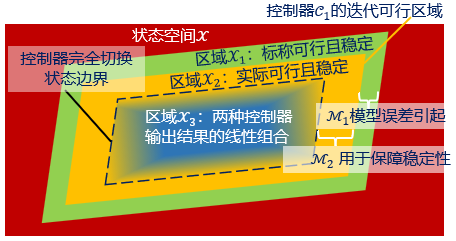
\includegraphics[width=0.6\linewidth]{fig/appx/controller_nesting.png}
      \caption{控制器嵌套方法的状态空间划分}
      \label{fig:controller_nesting}
    \end{figure}

    \begin{theorem}[控制器嵌套的稳定性]
    设车辆闭环系统为$\dot{\bm{x}} = f(\bm{x}, u)$，其中$\bm{x} \in \mathcal{X} \subseteq \mathbb{R}^n$为系统状态，$u \in \mathcal{U} \subseteq \mathbb{R}^m$为控制输入，$f: \mathcal{X} \times \mathcal{U} \to \mathbb{R}^n$满足局部利普希茨连续。若：
    1) 基础控制器$\mathcal{C}_1$使得闭环系统$\dot{\bm{x}} = f(\bm{x}, \mathcal{C}_1(\bm{x}))$在$\mathcal{X}_2$内李雅普诺夫稳定，即存在李雅普诺夫函数$V: \mathcal{X}_2 \to \mathbb{R}_{\geq 0}$，满足$\dot{V}(\bm{x}) = \nabla V(\bm{x})^T f(\bm{x}, \mathcal{C}_1(\bm{x})) \leq 0, \forall \bm{x} \in \mathcal{X}_2$；
    2) 加权系数$\alpha(\bm{x})$在$\mathcal{X}$上连续，且$\alpha(\bm{x}) = 1, \forall \bm{x} \in \mathcal{X}_2$；
    则：
    a) 嵌套控制器$\mathcal{C}_{\text{CN}}$下的闭环系统$\dot{\bm{x}} = f(\bm{x}, \mathcal{C}_{\text{CN}}(\bm{x}))$在$\mathcal{X}$内李雅普诺夫稳定；
    b) 当且仅当$\mathcal{C}_2$使得$\dot{V}(\bm{x}) = \nabla V(\bm{x})^T f(\bm{x}, \mathcal{C}_2(\bm{x})) < 0, \forall \bm{x} \in \mathcal{X}_3 \setminus \{\bm{x}^*\}$（$\bm{x}^*$为系统平衡点）时，$\mathcal{C}_{\text{CN}}$下的系统在$\mathcal{X}$内渐进稳定。
    \end{theorem}

    \begin{proof}
    \textbf{步骤1：证明李雅普诺夫稳定性（结论a）}
    由前提条件，$\mathcal{C}_1$对应的闭环系统在$\mathcal{X}_2$内存在李雅普诺夫函数$V(\bm{x})$，满足：
    $$\dot{V}(\bm{x}) = \nabla V(\bm{x})^T f(\bm{x}, \mathcal{C}_1(\bm{x})) \leq 0, \forall \bm{x} \in \mathcal{X}_2.$$
    对于$\mathcal{X}_3$区域，嵌套控制器输出为$\mathcal{C}_{\text{CN}}(\bm{x}) = \alpha\mathcal{C}_1 + (1-\alpha)\mathcal{C}_2$，其中$\alpha \in (0,1)$。由于$f(\bm{x}, u)$满足局部利普希茨连续，且$\mathcal{C}_1, \mathcal{C}_2$的输出均属于约束集$\mathcal{U}_{\text{con}}$，则$f(\bm{x}, \mathcal{C}_{\text{CN}}(\bm{x}))$可表示为：
    $$f(\bm{x}, \mathcal{C}_{\text{CN}}(\bm{x})) = \alpha f(\bm{x}, \mathcal{C}_1) + (1-\alpha) f(\bm{x}, \mathcal{C}_2).$$
    因此，李雅普诺夫函数的导数为：
    $$\dot{V}(\bm{x}) = \alpha \nabla V^T f(\bm{x}, \mathcal{C}_1) + (1-\alpha) \nabla V^T f(\bm{x}, \mathcal{C}_2).$$
    结合$\alpha \in (0,1)$且$\nabla V^T f(\bm{x}, \mathcal{C}_1) \leq 0$，同时$\mathcal{M}_1$补偿了模型误差，使得$\nabla V^T f(\bm{x}, \mathcal{C}_2)$在$\mathcal{X}_3$内有界且非正（$\nabla V^T f(\bm{x}, \mathcal{C}_2) \leq K, K < +\infty$），故$\dot{V}(\bm{x}) \leq 0, \forall \bm{x} \in \mathcal{X}$。
    根据李雅普诺夫稳定性判定定理，嵌套控制器下的系统在$\mathcal{X}$内李雅普诺夫稳定，且状态$\bm{x}(t)$无法脱离$\mathcal{X}_2$（最坏情况下在$\mathcal{M}_2$内震荡）。

    \textbf{步骤2：证明渐进稳定性的充要条件（结论b）}
    \textit{必要性}：若$\mathcal{C}_{\text{CN}}$下的系统渐进稳定，则$\dot{V}(\bm{x}) < 0, \forall \bm{x} \in \mathcal{X} \setminus \{\bm{x}^*\}$。
    对于$\mathcal{X}_2$区域，$\alpha = 1$，故$\dot{V}(\bm{x}) = \nabla V^T f(\bm{x}, \mathcal{C}_1) \leq 0$；
    对于$\mathcal{X}_3$区域，需满足$\dot{V}(\bm{x}) < 0$，即：
    $$\alpha \nabla V^T f(\bm{x}, \mathcal{C}_1) + (1-\alpha) \nabla V^T f(\bm{x}, \mathcal{C}_2) < 0.$$
    由于$\alpha \in (0,1)$且$\nabla V^T f(\bm{x}, \mathcal{C}_1) \leq 0$，则必须有$\nabla V^T f(\bm{x}, \mathcal{C}_2) < 0, \forall \bm{x} \in \mathcal{X}_3 \setminus \{\bm{x}^*\}$。

    \textit{充分性}：若$\nabla V^T f(\bm{x}, \mathcal{C}_2) < 0, \forall \bm{x} \in \mathcal{X}_3 \setminus \{\bm{x}^*\}$，则：
    $$\dot{V}(\bm{x}) = \alpha \nabla V^T f(\bm{x}, \mathcal{C}_1) + (1-\alpha) \nabla V^T f(\bm{x}, \mathcal{C}_2) < 0, \forall \bm{x} \in \mathcal{X} \setminus \{\bm{x}^*\}.$$
    根据渐进稳定的李雅普诺夫判定准则，系统在$\mathcal{X}$内渐进稳定。

    综上，定理的两个结论均得证。
    \end{proof}

    当内部嵌套的控制器$\mathcal{C}_2$为人类驾驶员（记为$\mathcal{C}_{\text{human}}$）时，控制器嵌套方法退化为辅助驾驶的稳域包裹（Stable Domain Wrapper, SD Wrapper）技术，其核心挑战可量化为：
    1) 状态空间的维度选择：需确定$\mathcal{X} = [x_1, x_2, ..., x_n]^T$中$n$的取值及各状态变量$x_i$的物理意义（如侧倾角、横摆角速度等）；
    2) 边界的数学表征：需通过优化方法求解$\mathcal{X}_2$的边界函数$\partial \mathcal{X}_2: g(\bm{x}) = 0$，及控制器切换的阈值$\alpha^* = \inf\{\alpha(\bm{x}) | \bm{x} \in \partial \mathcal{X}_3\}$。
    这两部分内容将作为后续研究推广过程的重点方向之一。


\section{插图}

% 附录中的插图示例（图~\ref{fig:appendix-figure}）。


  \begin{figure}
    \centering  
    \makebox[\linewidth]{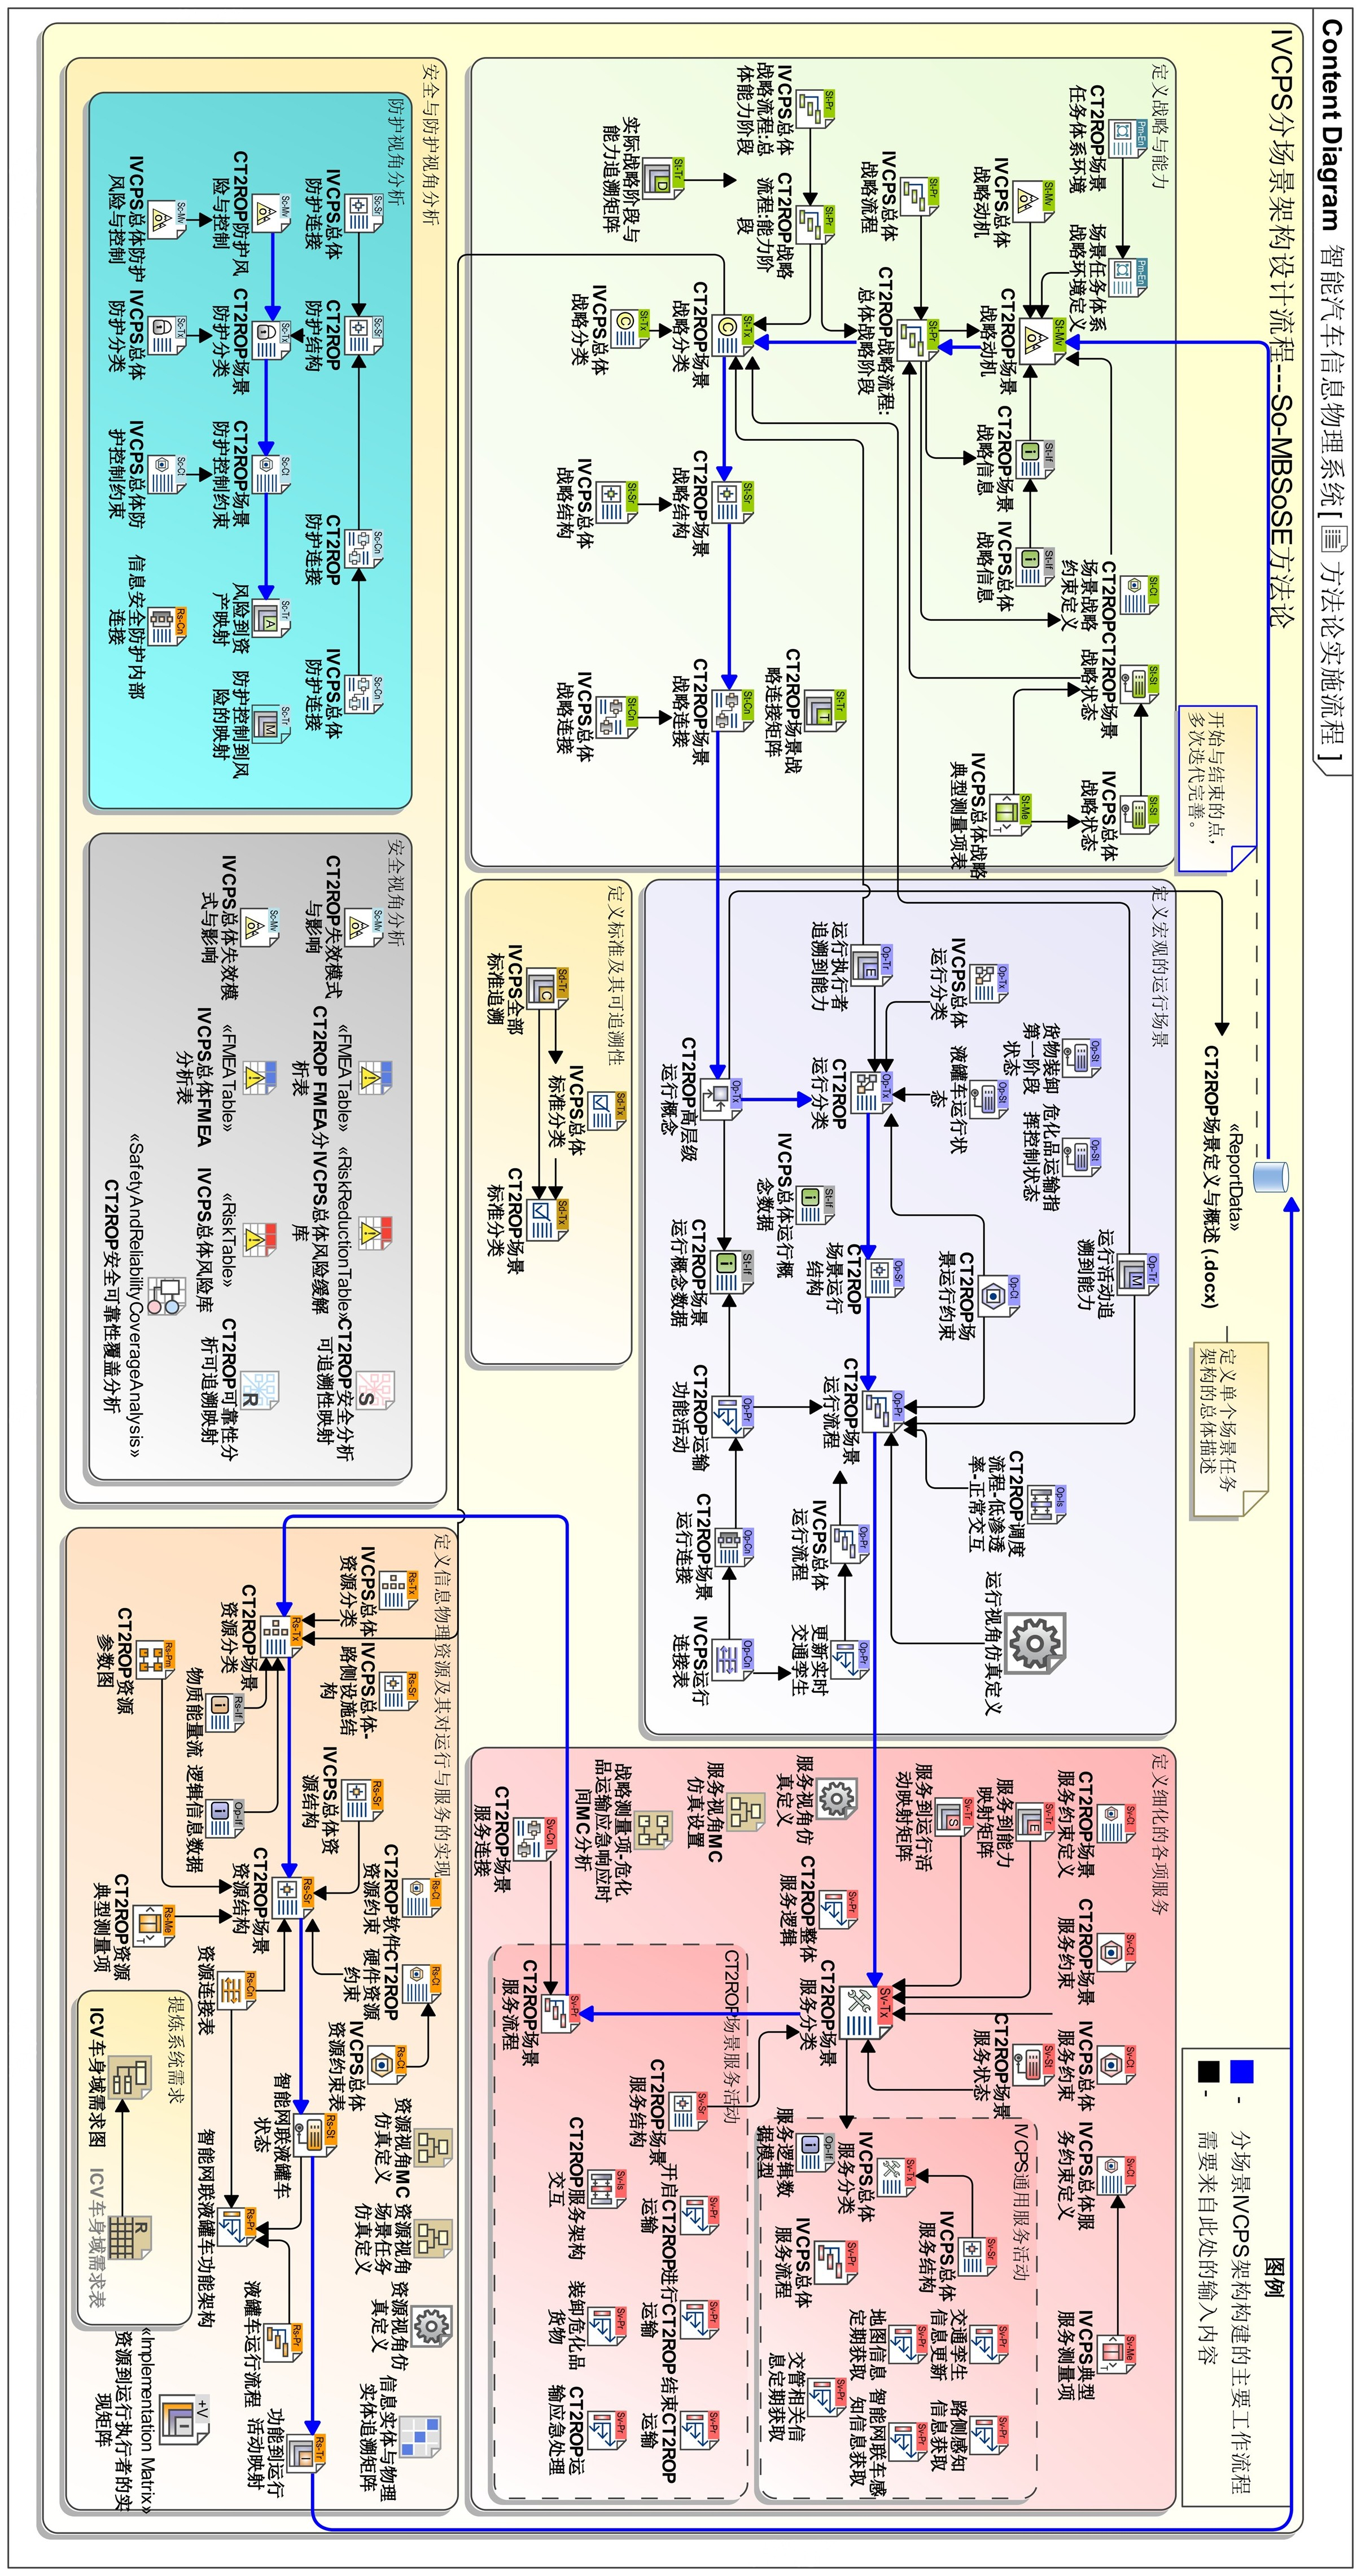
\includegraphics[width=0.8\linewidth]{fig/chap2/arch_process.jpg}}
    % \caption*{图片注释解释说明}
    \caption{车云协同危化品运输场景下IVCPS架构设计流程}
    \label{fig:arch_process}
  \end{figure} 

  \begin{figure}
    \centering 
    \makebox[\linewidth]{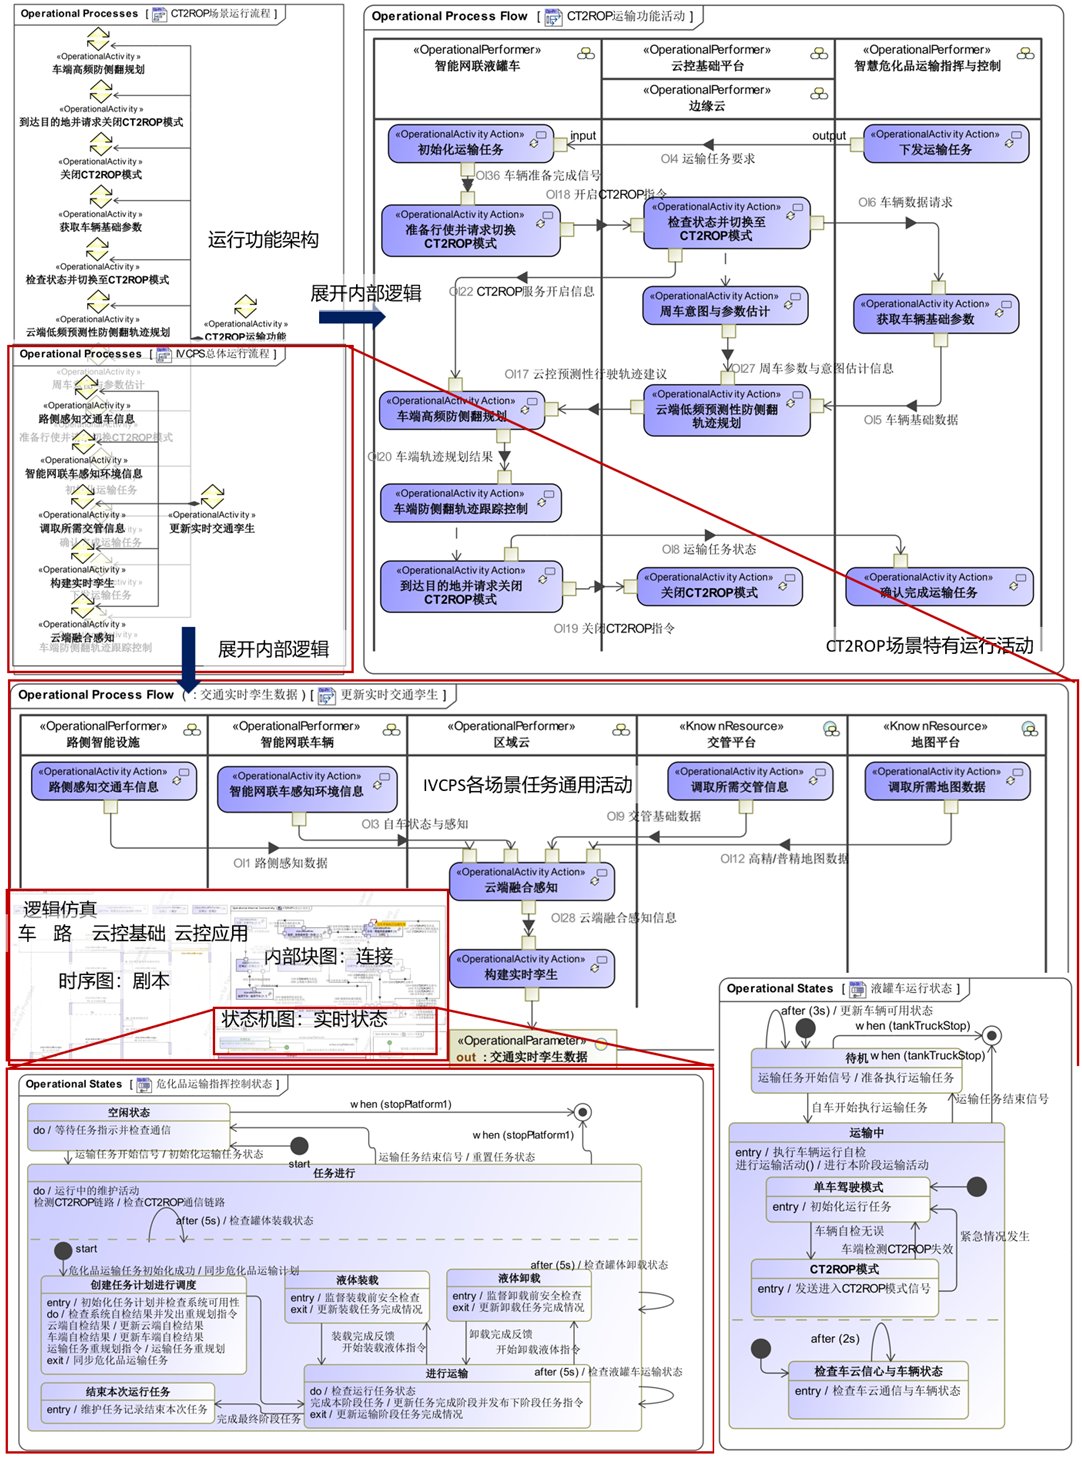
\includegraphics[width=1.0\linewidth]{fig/chap2/operation_sim.png}}
    % \caption*{图片注释解释说明}
    \caption{CT2ROP运行功能与逻辑行为及其仿真}
    \label{fig:operation_sim}
  \end{figure} 

  \begin{figure}
    \centering
    \makebox[\linewidth]{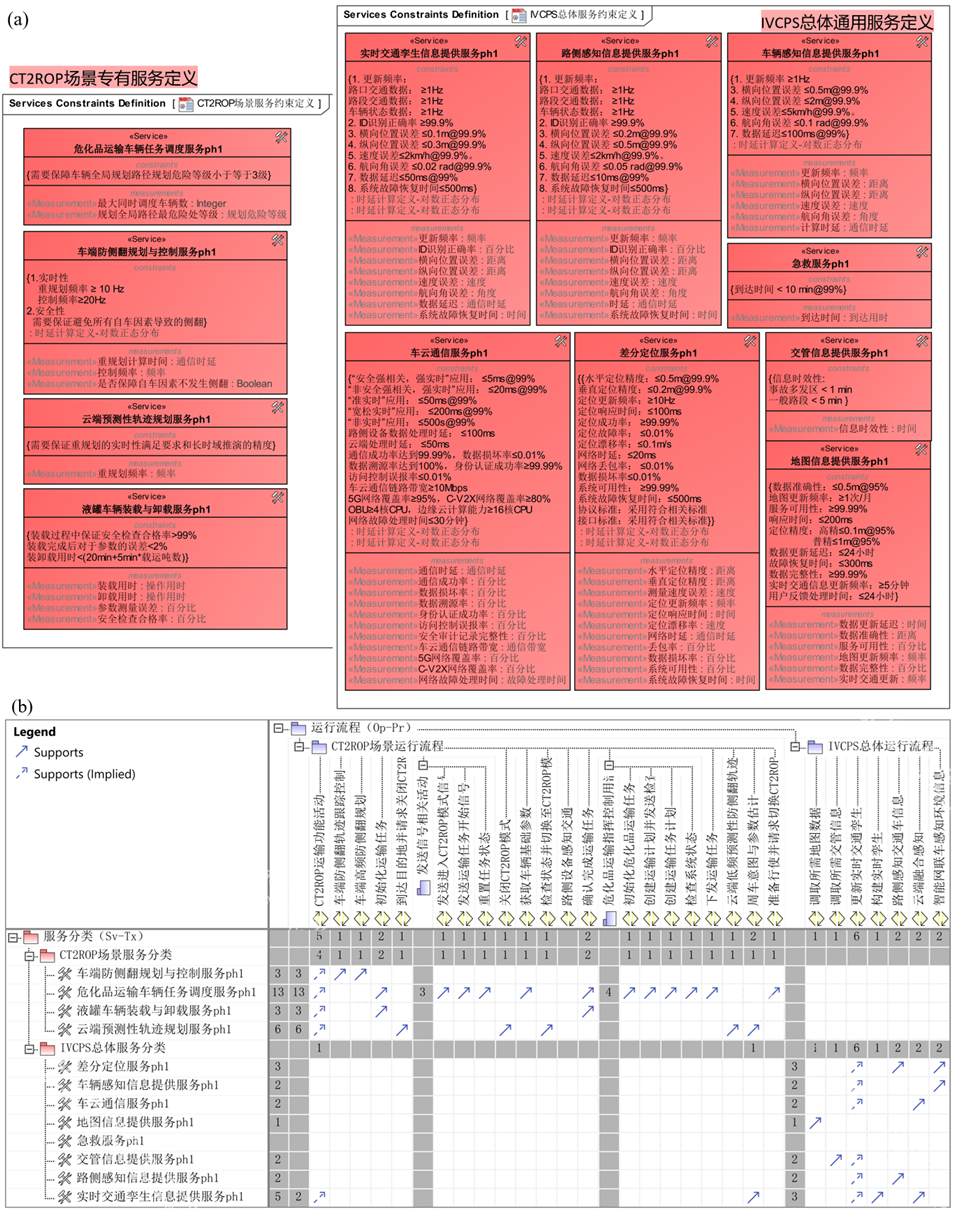
\includegraphics[width=1.0\linewidth]{fig/chap2/service_model.png}}
    \caption*{(a)服务约束视图下定义的CT2ROP专有服务及IVCPS通用服务 (b)所有服务与运行活动间的追溯关系}
    \caption{CT2ROP服务定义及其与运行活动追溯}
    \label{fig:service_model}
  \end{figure}

  \begin{figure}
    \centering 
    \makebox[\linewidth]{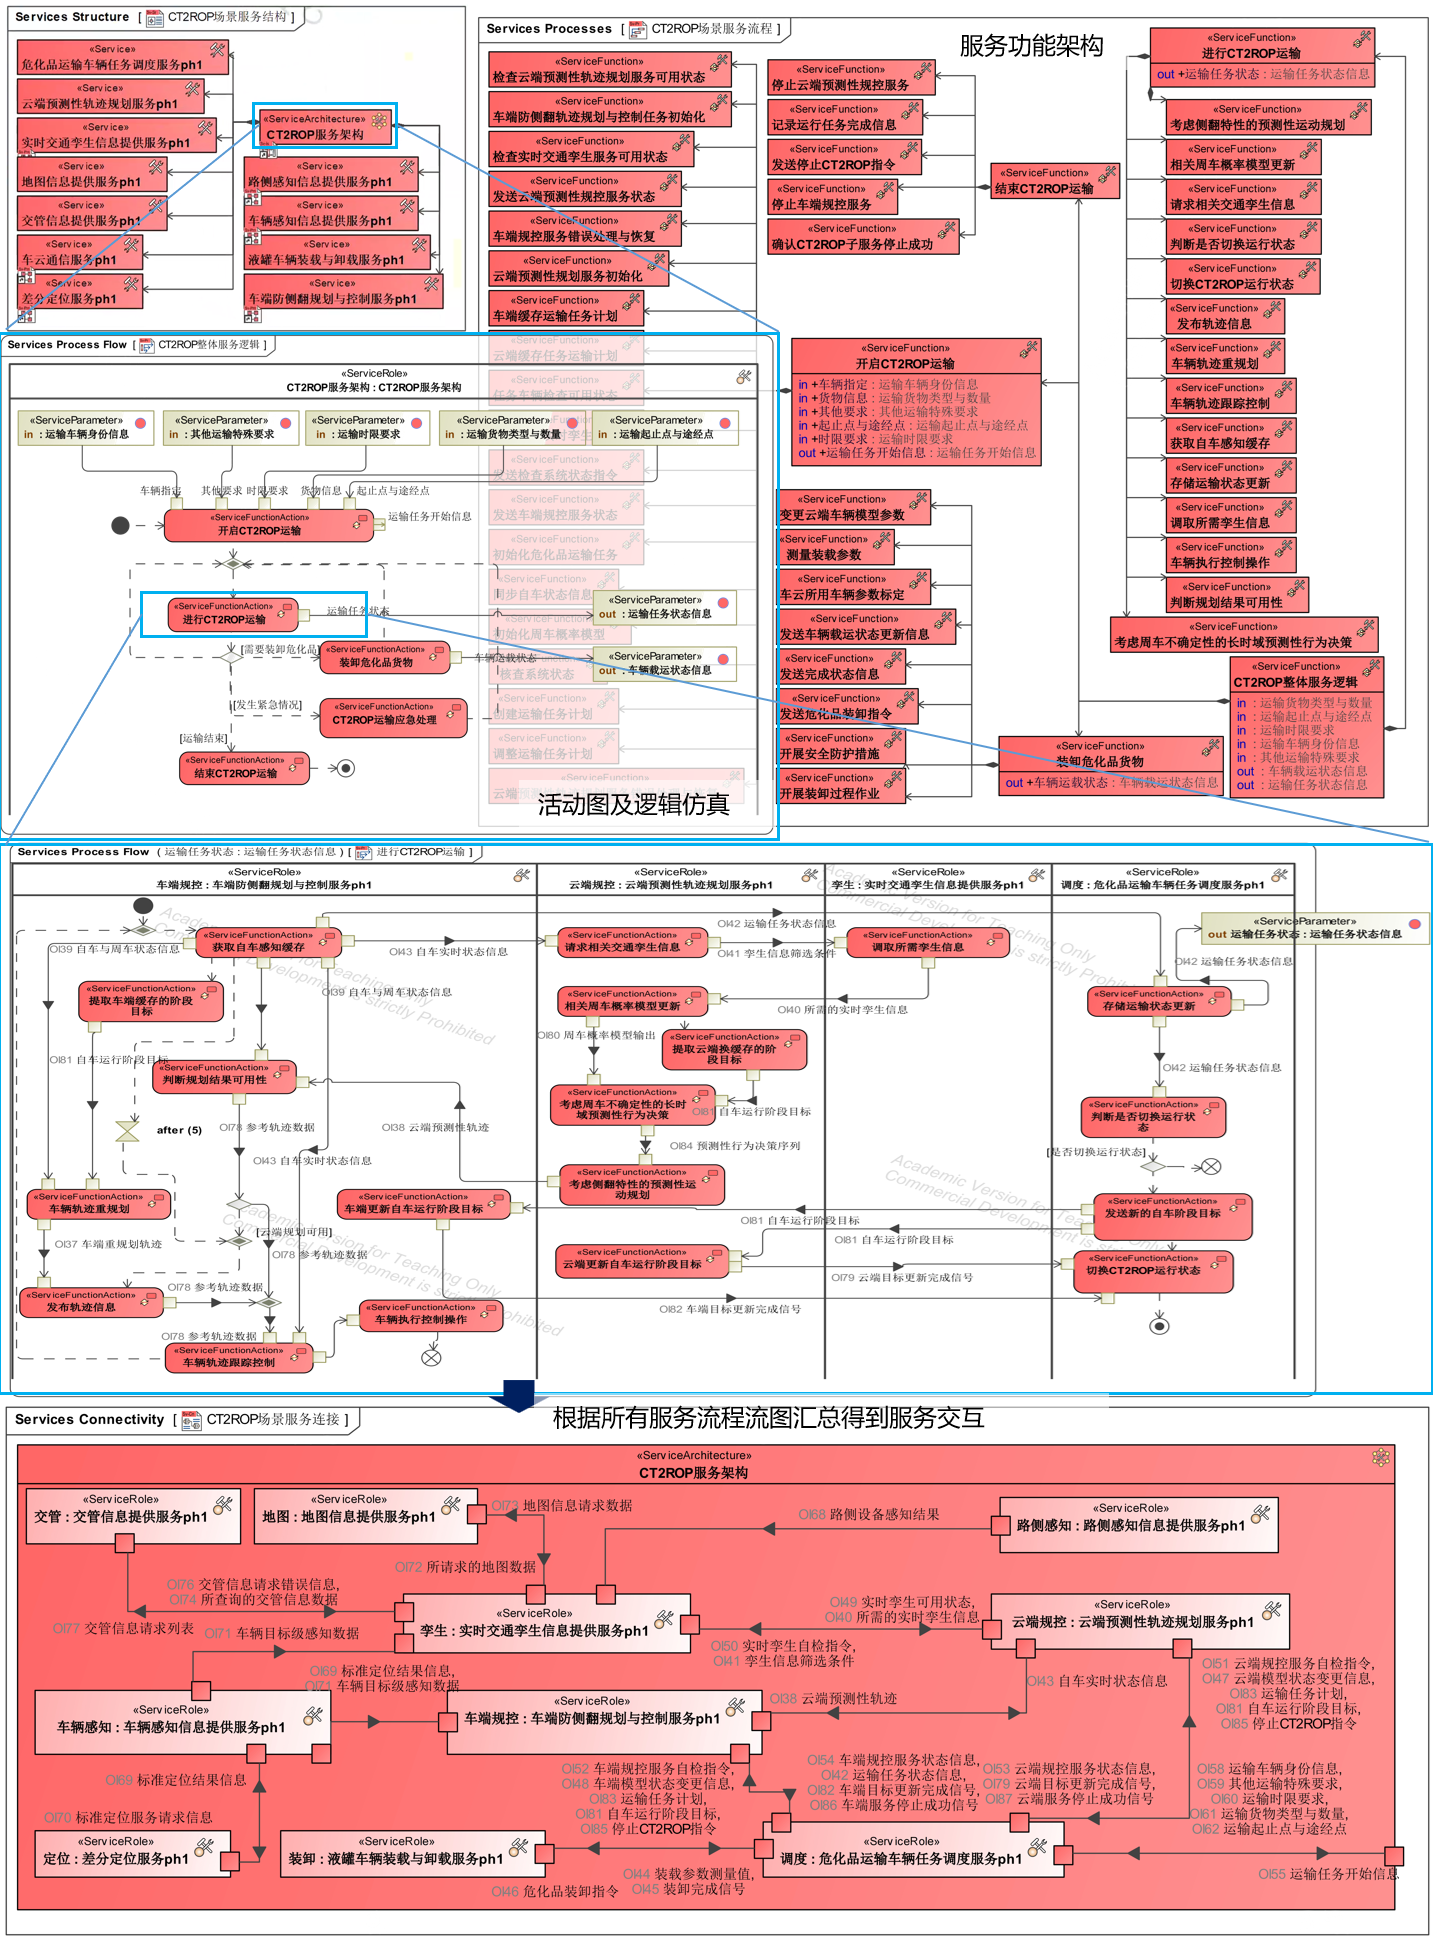
\includegraphics[width=1.0\linewidth]{fig/chap2/service_sim.png}}
    % \caption*{图片注释解释说明}
    \caption{CT2ROP服务功能与逻辑及其仿真}
    \label{fig:appendix_service_sim}
  \end{figure} 

  \begin{figure}
    \centering 
    \makebox[\linewidth]{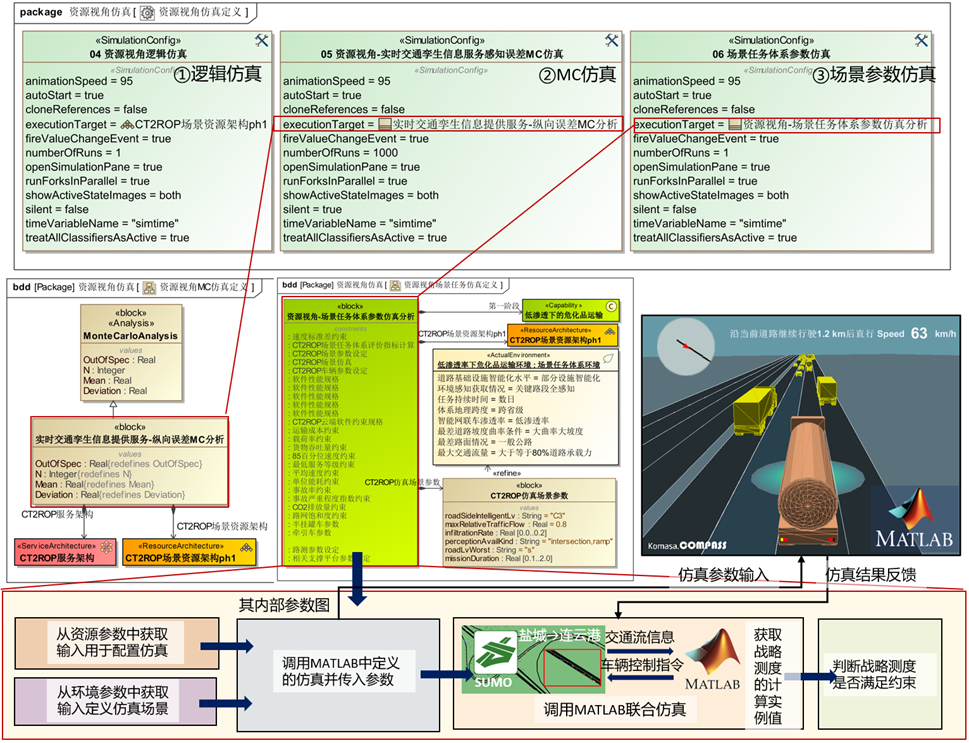
\includegraphics[width=1.0\linewidth]{fig/chap2/resource_sim.png}}
    % \caption*{图片注释解释说明}
    \caption{CT2ROP场景资源仿真分析}
    \label{fig:resource_sim}
  \end{figure} 

  \begin{figure}
  \centering
  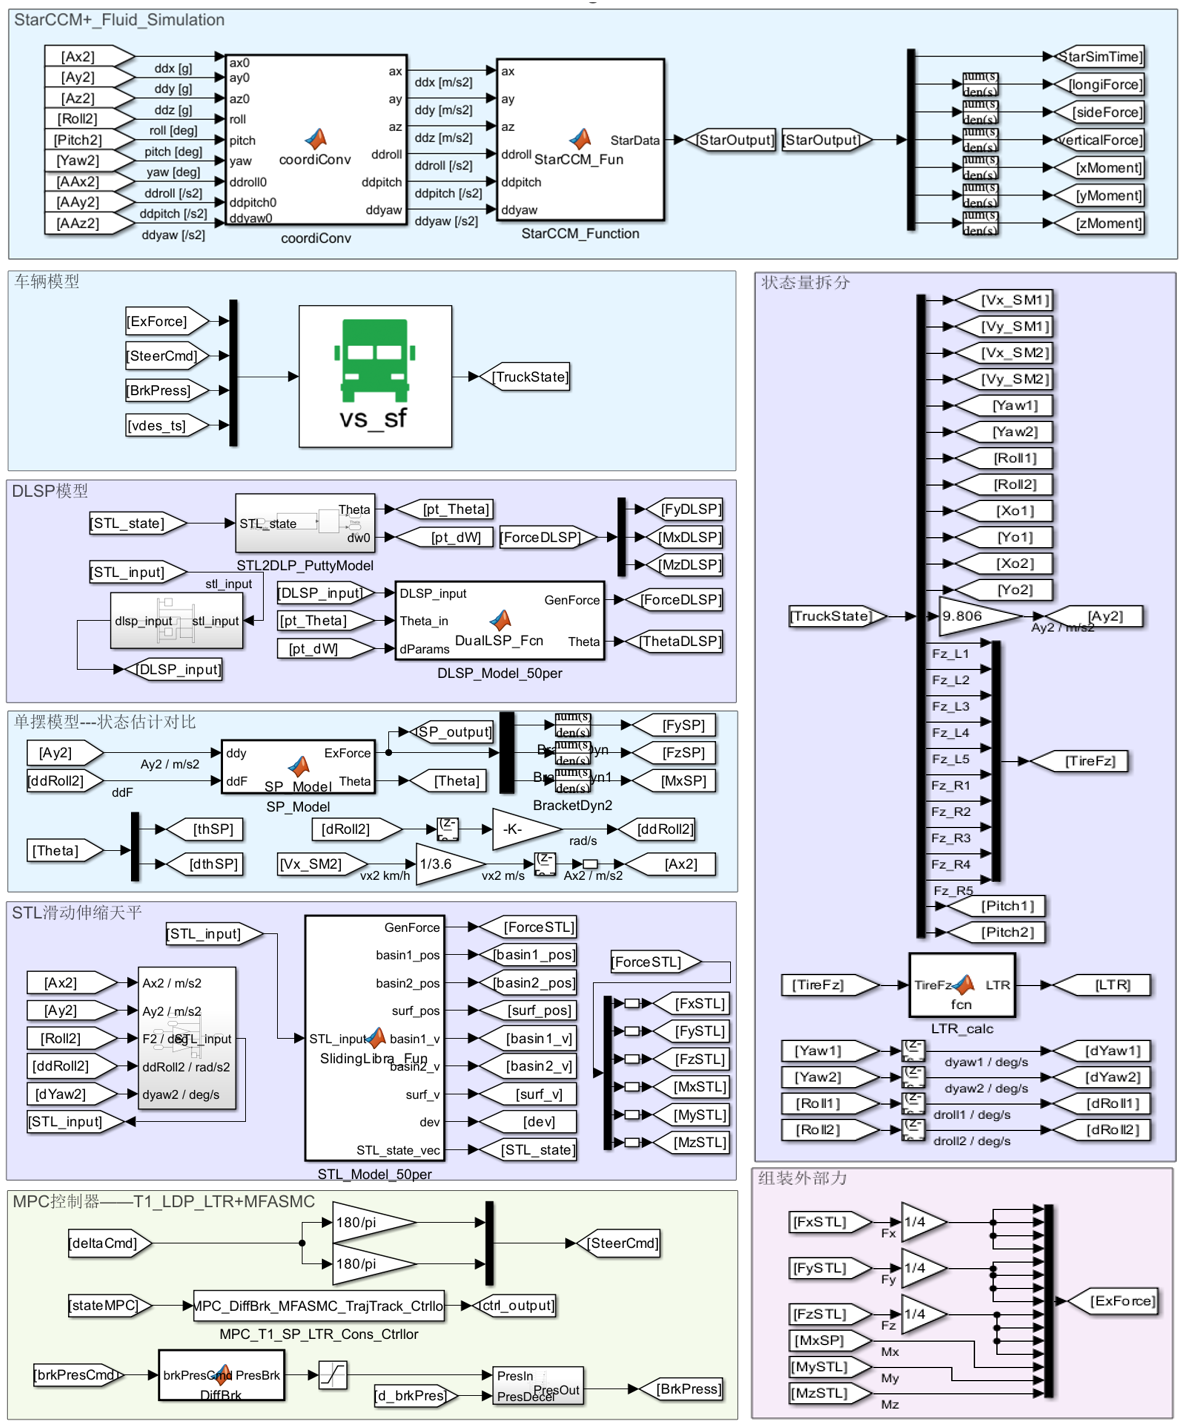
\includegraphics[width=1.0\linewidth]{fig/chap4/simulink_model.png}
  \caption{协同仿真平台Simulink模型}
  \label{fig:simulink_model}
  \end{figure}


  % \begin{figure}
  % \centering
  % 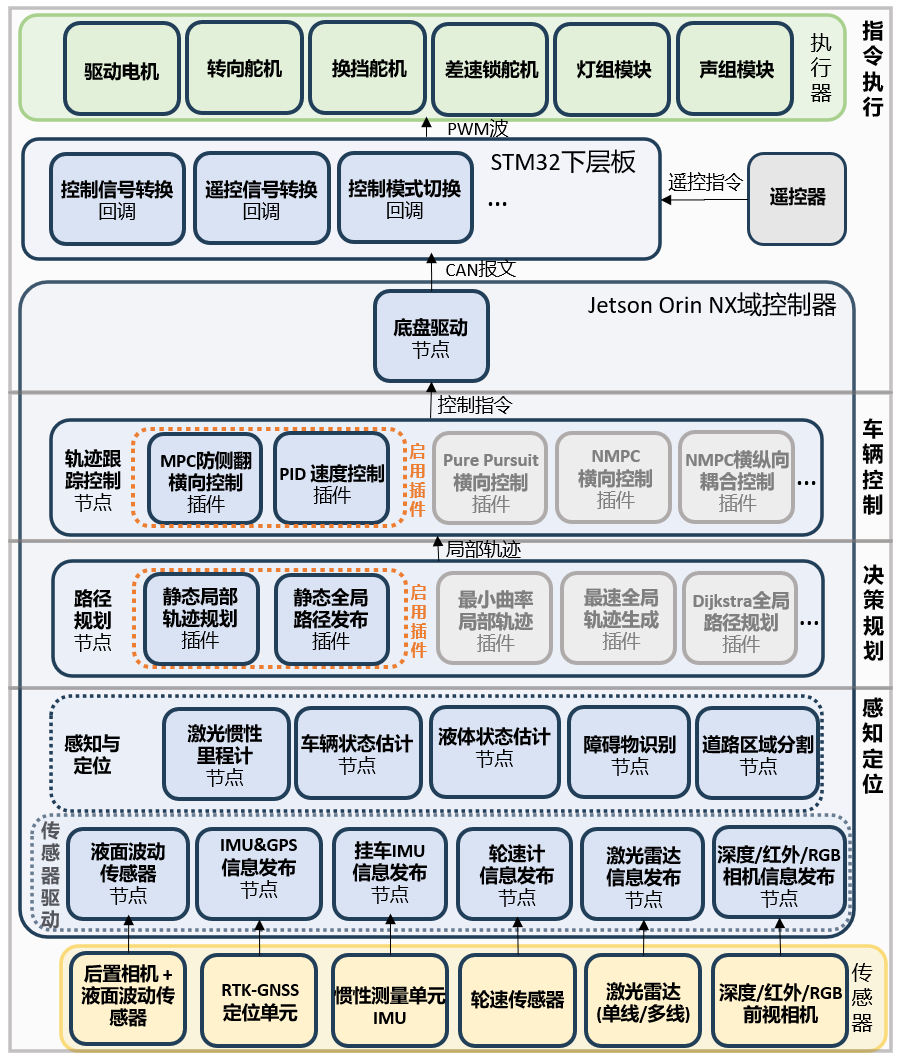
\includegraphics[width=0.8\linewidth]{fig/chap4/prog_arch.png}
  % \caption{自动驾驶软件架构}
  % \label{fig:prog_arch}
  % \end{figure}


\section{表格}

  % 附录中的表格示例（表~\ref{tab:appendix-table}）。

  {% 局部作用域，仅修改本表格式
  \small
  % \setlength{\tabcolsep}{3pt}       % 压缩列间距，节省横向空间（按要求注释）
  \renewcommand{\arraystretch}{1.0} 
  \linespread{0.7}\selectfont       % 强制锁定行高为0.7（按要求设置）

  \begin{longtable}{X c c c c c c c c c c l}  % 最后一列新增「用途」列
      \caption{仿真训练与验证场景设置}
      \label{tab:condition_table_all} \\
      \toprule
      路口 & 序号 & 名称 & $t_{depr}$ & $t_{start}$ & 终止点 & $q_{main}$ & $q_{merge}$ & $q_{exit}$ & $q_{avg}$ & 用途 \\
      \midrule
  \endfirsthead
      \caption*{续表~\thetable\quad 仿真训练与验证场景设置} \\
      \toprule
      路口 & 序号 & 名称 & $t_{depr}$ & $t_{start}$ & 终止点 & $q_{main}$ & $q_{merge}$ & $q_{exit}$ & $q_{avg}$ & 用途 \\
      \midrule
  \endhead
      \bottomrule
  \endfoot

  %-------------------------------------------------------------------------------
  % No.1（验证场景）
  \multirow{4}{*}{No.1} 
  & 1 & pass\_1 & 280 & 287 & $(3377,125023)$ & 2250 & 1125 & 1125 & 4500 & 验证 \\
  & 2 & merge\_1 & 120 & 230 & $(3377,125023)$ & 2250 & 1125 & 1125 & 4500 & 验证 \\
  & 3 & exit\_1 & 120 & 140 & $(1353,127222)$ & 2250 & 1125 & 1125 & 4500 & 验证 \\
  & 4 & cruise\_1 & 120 & 210 & $(6628,122202)$ & 2250 & 1125 & 1125 & 4500 & 验证 \\
  \midrule

  %-------------------------------------------------------------------------------
  % No.2（验证场景）
  \multirow{4}{*}{No.2} 
  & 5 & pass\_2 & 50 & 150 & $(8827,121224)$ & 2000 & 1000 & 1000 & 4000 & 验证 \\
  & 6 & merge\_2 & 120 & 125 & $(8827,121224)$ & 2000 & 1000 & 1000 & 4500 & 验证 \\
  & 7 & exit\_2 & 120 & 190 & $(7084,121972)$ & 2000 & 1000 & 1000 & 4500 & 验证 \\
  & 8 & cruise\_2 & 120 & 225 & $(13358,119455)$ & 2000 & 1000 & 1000 & 4500 & 验证 \\
  \midrule

  %-------------------------------------------------------------------------------
  % No.3（验证场景）
  \multirow{4}{*}{No.3} 
  & 9 & pass\_3 & 100 & 145 & $(15097,118843)$ & 1750 & 875 & 875 & 3500 & 验证 \\
  & 10 & merge\_3 & 100 & 160 & $(15097,118843)$ & 1750 & 875 & 875 & 3500 & 验证 \\
  & 11 & exit\_3 & 100 & 120 & $(13647,119360)$ & 1750 & 875 & 875 & 3500 & 验证 \\
  & 12 & cruise\_3 & 100 & 450 & $(26200,113761)$ & 1750 & 875 & 875 & 3500 & 验证 \\
  \midrule

  %-------------------------------------------------------------------------------
  % No.4（验证场景）
  \multirow{4}{*}{No.4} 
  & 13 & pass\_4 & 150 & 160 & $(35853,108391)$ & 1500 & 750 & 750 & 3000 & 验证 \\
  & 14 & merge\_4 & 150 & 185 & $(35853,108391)$ & 1500 & 750 & 750 & 3000 & 验证 \\
  & 15 & exit\_4 & 150 & 190 & $(34593,108938)$ & 1500 & 750 & 750 & 3000 & 验证 \\
  & 16 & cruise\_4 & 150 & 250 & $(42564,102705)$ & 1500 & 750 & 750 & 3000 & 验证 \\
  \midrule

  %-------------------------------------------------------------------------------
  % No.5（验证场景）
  \multirow{4}{*}{No.5} 
  & 17 & pass\_5 & 150 & 165 & $(44006,101780)$ & 1250 & 625 & 625 & 2500 & 验证 \\
  & 18 & merge\_5 & 150 & 230 & $(44004,101780)$ & 1250 & 625 & 625 & 2500 & 验证 \\
  & 19 & exit\_5 & 150 & 160 & $(43231,02663)$ & 1250 & 625 & 625 & 2500 & 验证 \\
  & 20 & cruise\_5 & 150 & 240 & $(49888,07671)$ & 1250 & 625 & 625 & 2500 & 验证 \\
  \midrule

  %-------------------------------------------------------------------------------
  % No.6（验证场景）
  \multirow{4}{*}{No.6} 
  & 21 & pass\_6 & 150 & 190 & $(51242,95154)$ & 1000 & 500 & 500 & 2000 & 验证 \\
  & 22 & merge\_6 & 150 & 155 & $(51242,95154)$ & 1000 & 500 & 500 & 2000 & 验证 \\
  & 23 & exit\_6 & 150 & 160 & $(50189,96489)$ & 1000 & 500 & 500 & 2000 & 验证 \\
  & 24 & cruise\_6 & 150 & 220 & $(58738,87984)$ & 1000 & 500 & 500 & 2000 & 验证 \\
  \midrule

  %-------------------------------------------------------------------------------
  % No.7（验证场景）
  \multirow{4}{*}{No.7} 
  & 25 & pass\_7 & 150 & 170 & $(60200,86293)$ & 750 & 375 & 375 & 1500 & 验证 \\
  & 26 & merge\_7 & 150 & 160 & $(60200,86293)$ & 750 & 375 & 375 & 1500 & 验证 \\
  & 27 & exit\_7 & 150 & 310 & $(59676,78847)$ & 750 & 375 & 375 & 1500 & 验证 \\
  & 28 & cruise\_7 & 150 & 310 & $(69330,89515)$ & 750 & 375 & 375 & 1500 & 验证 \\
  \midrule

  %-------------------------------------------------------------------------------
  % No.8（训练场景）
  \multirow{4}{*}{No.8} 
  & 29 & pass\_8 & 100 & 130 & $(70907,78147)$ & 1250 & 1125 & 1125 & 4500 & 训练 \\
  & 30 & merge\_8 & 100 & 130 & $(70907,78147)$ & 1250 & 1125 & 1125 & 4500 & 训练 \\
  & 31 & exit\_8 & 100 & 130 & $(69498,79025)$ & 1250 & 1125 & 1125 & 4500 & 训练 \\
  & 32 & cruise\_8 & 100 & 130 & $(74891,72481)$ & 1250 & 1125 & 1125 & 4500 & 训练 \\
  \midrule

  %-------------------------------------------------------------------------------
  % No.9（训练场景）
  \multirow{4}{*}{No.9} 
  & 33 & pass\_9 & 120 & 150 & $(75573,70800)$ & 2000 & 1000 & 1000 & 4000 & 训练 \\
  & 34 & merge\_9 & 120 & 150 & $(75573,70800)$ & 2000 & 1000 & 1000 & 4000 & 训练 \\
  & 35 & exit\_9 & 120 & 150 & $(74896,71940)$ & 2000 & 1000 & 1000 & 4000 & 训练 \\
  & 36 & cruise\_9 & 120 & 150 & $(85038,58160)$ & 2000 & 1000 & 1000 & 4000 & 训练 \\
  \midrule

  %-------------------------------------------------------------------------------
  % No.10（训练场景）
  \multirow{4}{*}{No.10} 
  & 37 & pass\_10 & 100 & 130 & $(92050,46785)$ & 1750 & 875 & 875 & 3500 & 训练 \\
  & 38 & merge\_10 & 100 & 130 & $(92050,46785)$ & 1750 & 875 & 875 & 3500 & 训练 \\
  & 39 & exit\_10 & 100 & 130 & $(92054,48293)$ & 1750 & 875 & 875 & 3500 & 训练 \\
  & 40 & cruise\_10 & 100 & 130 & $(96740,37970)$ & 1750 & 875 & 875 & 3500 & 训练 \\
  \midrule

  %-------------------------------------------------------------------------------
  % No.11（训练场景）
  \multirow{4}{*}{No.11} 
  & 41 & pass\_11 & 150 & 180 & $(98075,37971)$ & 1500 & 750 & 750 & 3000 & 训练 \\
  & 42 & merge\_11 & 150 & 180 & $(98075,37971)$ & 1500 & 750 & 750 & 3000 & 训练 \\
  & 43 & exit\_11 & 150 & 180 & $(97180,30472)$ & 1500 & 750 & 750 & 3000 & 训练 \\
  & 44 & cruise\_11 & 150 & 180 & $(34068,110111)$ & 1500 & 750 & 750 & 3000 & 训练 \\
  \midrule

  %-------------------------------------------------------------------------------
  % No.12（训练场景）
  \multirow{4}{*}{No.12} 
  & 45 & pass\_12 & 150 & 180 & $(99643,35167)$ & 1250 & 625 & 625 & 2500 & 训练 \\
  & 46 & merge\_12 & 150 & 180 & $(99643,35167)$ & 1250 & 625 & 625 & 2500 & 训练 \\
  & 47 & exit\_12 & 150 & 180 & $(98931,36237)$ & 1250 & 625 & 625 & 2500 & 训练 \\
  & 48 & cruise\_12 & 150 & 180 & $(104324,24317)$ & 1250 & 625 & 625 & 2500 & 训练 \\
  \midrule

  %-------------------------------------------------------------------------------
  % No.13（训练场景）
  \multirow{4}{*}{No.13} 
  & 49 & pass\_13 & 150 & 180 & $(104781,21843)$ & 1000 & 500 & 500 & 2000 & 训练 \\
  & 50 & merge\_13 & 150 & 180 & $(104781,21843)$ & 1000 & 500 & 500 & 2000 & 训练 \\
  & 51 & exit\_13 & 150 & 180 & $(104332,22626)$ & 1000 & 500 & 500 & 2000 & 训练 \\
  & 52 & cruise\_13 & 150 & 180 & $(107112,14877)$ & 1000 & 500 & 500 & 2000 & 训练 \\
  \midrule

  %-------------------------------------------------------------------------------
  % No.14（训练场景）
  \multirow{4}{*}{No.14} 
  & 53 & pass\_14 & 150 & 180 & $(107705,13226)$ & 750 & 375 & 375 & 1500 & 训练 \\
  & 54 & merge\_14 & 150 & 180 & $(107705,13226)$ & 750 & 375 & 375 & 1500 & 训练 \\
  & 55 & exit\_14 & 150 & 180 & $(107203,14112)$ & 750 & 375 & 375 & 1500 & 训练 \\
  & 56 & cruise\_14 & 150 & 180 & $(111286,6653)$ & 750 & 375 & 375 & 1500 & 训练 \\
  \midrule

  %-------------------------------------------------------------------------------
  % No.15（训练场景）
  \multirow{4}{*}{No.15} 
  & 57 & pass\_15 & 150 & 180 & $(112301,4704)$ & 500 & 250 & 250 & 1000 & 训练 \\
  & 58 & merge\_15 & 150 & 180 & $(112301,4704)$ & 500 & 250 & 250 & 1000 & 训练 \\
  & 59 & exit\_15 & 150 & 180 & $(111604,5761)$ & 500 & 250 & 250 & 1000 & 训练 \\
  & 60 & cruise\_15 & 150 & 180 & $(108764,3804)$ & 500 & 250 & 250 & 1000 & 训练 \\

  \end{longtable}
  }% 结束局部作用域




  {% 局部作用域，仅修改本表格式，不影响全文
  \small
  % \setlength{\tabcolsep}{3pt}       % 压缩列间距，节省横向空间
  \renewcommand{\arraystretch}{1.0} % 恢复紧凑行距，解决longtable行距过大问题
  \linespread{0.7}\selectfont       % 强制锁定行高

  \begin{longtable}{l l c c c}
      \caption{交通流仿真分任务得分情况 (mean $\pm$ SEM)}
      \label{tab:reward_task} \\
      \toprule
      Task & Reward term & IDM+MOBIL & TreeSearch & Graphflow \\
      \midrule
  \endfirsthead
      \caption*{续表~\thetable\quad 交通流仿真分任务得分情况 (mean $\pm$ SEM)} \\
      \toprule
      Task & Reward term & IDM+MOBIL & TreeSearch & Graphflow \\
      \midrule
  \endhead
      \bottomrule
  \endfoot

  %-------------------------------------------------------------------------------
  \multirow{9}{*}{Task 1}
  & Safe-1/TTC       & -4.04$\pm$0.42 & -3.84$\pm$0.27 & \textbf{-3.59$\pm$0.23} \\
  & Safe-MEI         & -16.14$\pm$9.55 & -2.17$\pm$0.52 & \textbf{-1.69$\pm$0.37} \\
  & Safe-RTTC        & -0.93$\pm$0.14 & -0.91$\pm$0.12 & \textbf{-0.68$\pm$0.11} \\
  & Safe-1/HW        & -82.65$\pm$8.03 & -62.00$\pm$4.84 & \textbf{-54.74$\pm$3.93} \\
  & \textbf{Safe Reward} & -103.76$\pm$12.56 & -68.92$\pm$5.12 & \textbf{-60.70$\pm$4.27} \\
  & \textbf{Effi Reward} & 183.15$\pm$5.03 & 198.16$\pm$5.58 & \textbf{198.75$\pm$5.39} \\
  & Navi-Lane        & \textbf{22.53$\pm$1.00} & 21.67$\pm$0.78 & 21.86$\pm$0.75 \\
  & Navi-Mission     & 2.86$\pm$2.01 & 88.57$\pm$3.83 & \textbf{95.71$\pm$2.44} \\
  & \textbf{Navi Reward} & 25.39$\pm$2.36 & 110.24$\pm$3.84 & \textbf{117.57$\pm$2.58} \\
  & \textbf{Comf Reward} & -19.39$\pm$0.94 & -18.34$\pm$0.68 & \textbf{-18.27$\pm$0.68} \\
  & \textbf{Total Reward} & 85.38$\pm$13.46 & 221.13$\pm$7.27 & \textbf{237.35$\pm$6.02} \\
  \midrule

  %-------------------------------------------------------------------------------
  \multirow{10}{*}{Task 2}
  & Safe-1/TTC       & \textbf{-1.43$\pm$0.12} & -1.58$\pm$0.12 & -1.87$\pm$0.13 \\
  & Safe-MEI         & -26.79$\pm$11.12 & \textbf{-1.51$\pm$0.25} & -2.99$\pm$0.84 \\
  & Safe-RTTC        & -0.99$\pm$0.09 & \textbf{-0.73$\pm$0.07} & -0.82$\pm$0.08 \\
  & Safe-1/HW        & -35.22$\pm$3.25 & -18.90$\pm$2.28 & \textbf{-17.45$\pm$2.44} \\
  & \textbf{Safe Reward} & -64.44$\pm$11.14 & \textbf{-22.71$\pm$2.41} & -23.14$\pm$2.74 \\
  & \textbf{Effi Reward} & 110.80$\pm$6.37 & 114.58$\pm$5.97 & \textbf{116.03$\pm$6.08} \\
  & Navi-Lane        & 14.46$\pm$0.69 & 15.48$\pm$0.71 & \textbf{16.77$\pm$0.73} \\
  & Navi-Mission     & 97.14$\pm$2.01 & \textbf{100.00$\pm$0.00} & \textbf{100.00$\pm$0.00} \\
  & \textbf{Navi Reward} & 111.60$\pm$2.36 & 115.48$\pm$0.71 & \textbf{116.77$\pm$0.73} \\
  & \textbf{Rule Reward} & 25.15$\pm$2.30 & 26.19$\pm$2.19 & \textbf{26.31$\pm$2.39} \\
  & \textbf{Comf Reward} & -11.42$\pm$0.58 & \textbf{-11.11$\pm$0.56} & -11.18$\pm$0.54 \\
  & \textbf{Total Reward} & 171.70$\pm$14.83 & 222.42$\pm$6.43 & \textbf{224.80$\pm$7.27} \\
  \midrule

  %-------------------------------------------------------------------------------
  \multirow{11}{*}{Task 3}
  & Safe-1/TTC       & -3.10$\pm$0.17 & \textbf{-2.82$\pm$0.14} & -3.16$\pm$0.18 \\
  & Safe-MEI         & -12.42$\pm$5.45 & \textbf{-0.90$\pm$0.14} & -1.37$\pm$0.29 \\
  & Safe-RTTC        & -0.61$\pm$0.08 & \textbf{-0.26$\pm$0.04} & -0.39$\pm$0.06 \\
  & Safe-1/HW        & -41.23$\pm$3.13 & \textbf{-24.28$\pm$2.14} & -27.34$\pm$2.35 \\
  & \textbf{Safe Reward} & -57.36$\pm$6.29 & \textbf{-28.26$\pm$2.19} & -32.25$\pm$2.44 \\
  & \textbf{Effi Reward} & 105.90$\pm$6.11 & 114.89$\pm$5.68 & \textbf{115.86$\pm$5.58} \\
  & Navi-Lane        & \textbf{15.77$\pm$0.66} & 14.74$\pm$0.58 & 15.59$\pm$0.65 \\
  & Navi-Mission     & 98.57$\pm$1.43 & \textbf{100.00$\pm$0.00} & \textbf{100.00$\pm$0.00} \\
  & \textbf{Navi Reward} & 114.34$\pm$1.69 & 114.74$\pm$0.58 & \textbf{115.59$\pm$0.65} \\
  & \textbf{Rule Reward} & \textbf{31.29$\pm$1.90} & 26.81$\pm$1.63 & 26.75$\pm$1.85 \\
  & \textbf{Comf Reward} & -12.85$\pm$0.46 & \textbf{-11.35$\pm$0.40} & -11.72$\pm$0.40 \\
  & \textbf{Total Reward} & \textbf{181.33$\pm$10.31} & 216.83$\pm$6.63 & 214.22$\pm$6.21 \\
  \midrule

  %-------------------------------------------------------------------------------
  \multirow{10}{*}{Task 4}
  & Safe-1/TTC       & -4.70$\pm$0.34 & \textbf{-4.10$\pm$0.26} & -4.38$\pm$0.29 \\
  & Safe-MEI         & -3.00$\pm$0.73 & -1.55$\pm$0.24 & \textbf{-1.38$\pm$0.17} \\
  & Safe-RTTC        & -0.70$\pm$0.13 & -0.62$\pm$0.07 & \textbf{-0.57$\pm$0.06} \\
  & Safe-1/HW        & -176.83$\pm$9.12 & \textbf{-135.01$\pm$7.39} & -141.76$\pm$7.12 \\
  & \textbf{Safe Reward} & -185.23$\pm$9.47 & \textbf{-141.28$\pm$7.59} & -148.09$\pm$7.25 \\
  & \textbf{Effi Reward} & 547.09$\pm$17.74 & \textbf{559.02$\pm$17.30} & 554.70$\pm$18.17 \\
  & Navi-Lane        & \textbf{46.24$\pm$1.54} & 45.86$\pm$1.49 & 46.09$\pm$1.60 \\
  & Navi-Mission     & 1.43$\pm$1.43 & 72.86$\pm$5.35 & \textbf{84.29$\pm$4.38} \\
  & \textbf{Navi Reward} & 47.67$\pm$2.16 & 118.72$\pm$4.68 & \textbf{130.37$\pm$3.63} \\
  & \textbf{Rule Reward} & 151.05$\pm$7.44 & \textbf{168.74$\pm$5.89} & 157.62$\pm$7.21 \\
  & \textbf{Comf Reward} & -46.06$\pm$1.47 & \textbf{-45.62$\pm$1.39} & -45.68$\pm$1.47 \\
  & \textbf{Total Reward} & 514.52$\pm$23.24 & \textbf{659.59$\pm$19.52} & 648.93$\pm$21.99 \\

  \end{longtable}
  }% 结束局部作用域，恢复全局格式



  {% 局部作用域，只改本表行距，不影响全文
  \small
  % \setlength{\tabcolsep}{3pt}       % 压缩列间距
  \renewcommand{\arraystretch}{1.0} % 核心：恢复正常紧凑行距
  \linespread{0.7}\selectfont       % 强制行高

  \begin{longtable}{l l c c c}
      \caption{交通流仿真分流量得分情况 (mean $\pm$ SEM)}
      \label{tab:reward_flow} \\
      \toprule
      Flow (veh/h) & Reward term & IDM+MOBIL & TreeSearch & Graphflow \\
      \midrule
  \endfirsthead
      \caption*{续表~\thetable\quad 交通流仿真分流量得分情况 (mean $\pm$ SEM)} \\
      \toprule
      Flow (veh/h) & Reward term & IDM+MOBIL & TreeSearch & Graphflow \\
      \midrule
  \endhead
      \bottomrule
  \endfoot

  %-------------------------------------------------------------------------------
  \multirow{11}{*}{4500}
  & Safe-1/TTC       & -4.47$\pm$0.71 & -3.57$\pm$0.44 & \textbf{-3.39$\pm$0.35} \\
  & Safe-MEI         & -2.75$\pm$0.80 & \textbf{-1.76$\pm$0.30} & -2.65$\pm$0.61 \\
  & Safe-RTTC        & -1.17$\pm$0.15 & \textbf{-0.92$\pm$0.12} & -1.00$\pm$0.13 \\
  & Safe-1/HW        & -121.10$\pm$12.19 & -79.61$\pm$9.10 & \textbf{-74.66$\pm$8.29} \\
  & \textbf{Safe Reward} & -129.48$\pm$13.10 & -85.86$\pm$9.27 & \textbf{-81.70$\pm$8.49} \\
  & \textbf{Effi Reward} & 224.15$\pm$20.62 & \textbf{257.37$\pm$21.30} & 248.41$\pm$19.29 \\
  & Navi-Lane        & \textbf{27.23$\pm$1.73} & 27.01$\pm$1.61 & 26.74$\pm$1.52 \\
  & Navi-Mission     & 52.50$\pm$8.00 & 90.00$\pm$4.80 & \textbf{97.50$\pm$2.50} \\
  & \textbf{Navi Reward} & 79.73$\pm$6.65 & 117.01$\pm$4.75 & \textbf{124.24$\pm$2.91} \\
  & \textbf{Rule Reward} & 49.18$\pm$7.87 & \textbf{58.28$\pm$9.30} & 51.02$\pm$7.97 \\
  & \textbf{Comf Reward} & -25.60$\pm$1.77 & -24.38$\pm$1.69 & \textbf{-23.76$\pm$1.58} \\
  & \textbf{Total Reward} & 197.98$\pm$28.37 & \textbf{322.41$\pm$26.71} & 318.21$\pm$22.10 \\
  \midrule

  %-------------------------------------------------------------------------------
  \multirow{10}{*}{4000}
  & Safe-1/TTC       & -3.13$\pm$0.30 & -2.92$\pm$0.28 & \textbf{-2.82$\pm$0.24} \\
  & Safe-MEI         & -19.19$\pm$8.29 & -2.74$\pm$0.83 & \textbf{-2.56$\pm$0.77} \\
  & Safe-RTTC        & -1.09$\pm$0.23 & \textbf{-0.74$\pm$0.10} & -0.80$\pm$0.11 \\
  & Safe-1/HW        & -92.12$\pm$8.08 & \textbf{-61.43$\pm$6.29} & -62.63$\pm$6.49 \\
  & \textbf{Safe Reward} & -115.53$\pm$10.11 & \textbf{-67.82$\pm$6.50} & -68.81$\pm$6.54 \\
  & \textbf{Effi Reward} & 183.22$\pm$15.37 & \textbf{198.06$\pm$15.70} & 193.86$\pm$14.40 \\
  & Navi-Lane        & \textbf{23.72$\pm$0.79} & 21.56$\pm$1.00 & 21.65$\pm$0.82 \\
  & Navi-Mission     & 50.00$\pm$8.01 & 95.00$\pm$3.49 & \textbf{100.00$\pm$0.00} \\
  & \textbf{Navi Reward} & 73.72$\pm$7.40 & 116.56$\pm$3.42 & \textbf{121.65$\pm$0.82} \\
  & \textbf{Rule Reward} & 37.20$\pm$4.82 & \textbf{41.14$\pm$6.07} & 35.77$\pm$5.02 \\
  & \textbf{Comf Reward} & -20.37$\pm$0.86 & \textbf{-18.86$\pm$1.06} & -19.14$\pm$0.91 \\
  & \textbf{Total Reward} & 158.24$\pm$12.92 & \textbf{269.08$\pm$17.18} & 263.32$\pm$13.17 \\
  \midrule

  %-------------------------------------------------------------------------------
  \multirow{10}{*}{3500}
  & Safe-1/TTC       & -2.90$\pm$0.26 & \textbf{-2.83$\pm$0.26} & -3.30$\pm$0.28 \\
  & Safe-MEI         & -63.06$\pm$24.50 & \textbf{-2.76$\pm$0.42} & -4.77$\pm$1.25 \\
  & Safe-RTTC        & -1.48$\pm$0.14 & -1.17$\pm$0.16 & \textbf{-1.11$\pm$0.14} \\
  & Safe-1/HW        & -84.28$\pm$13.73 & \textbf{-64.15$\pm$13.19} & -66.83$\pm$12.05 \\
  & \textbf{Safe Reward} & -151.72$\pm$25.27 & \textbf{-70.91$\pm$13.51} & -76.02$\pm$11.94 \\
  & \textbf{Effi Reward} & 217.74$\pm$35.59 & 227.23$\pm$34.80 & \textbf{229.37$\pm$34.92} \\
  & Navi-Lane        & 23.45$\pm$2.59 & 23.81$\pm$2.36 & \textbf{24.17$\pm$2.41} \\
  & Navi-Mission     & 45.00$\pm$7.97 & \textbf{95.00$\pm$3.49} & \textbf{95.00$\pm$3.49} \\
  & \textbf{Navi Reward} & 68.45$\pm$7.19 & 118.81$\pm$3.48 & \textbf{119.17$\pm$4.44} \\
  & \textbf{Rule Reward} & \textbf{55.01$\pm$12.00} & 53.43$\pm$11.61 & 53.35$\pm$12.12 \\
  & \textbf{Comf Reward} & -21.25$\pm$2.78 & \textbf{-20.82$\pm$2.63} & \textbf{-20.82$\pm$2.73} \\
  & \textbf{Total Reward} & 168.22$\pm$45.89 & \textbf{307.75$\pm$35.36} & 305.06$\pm$36.91 \\
  \midrule

  %-------------------------------------------------------------------------------
  \multirow{10}{*}{3000}
  & Safe-1/TTC       & -3.24$\pm$0.31 & \textbf{-2.96$\pm$0.28} & -3.27$\pm$0.28 \\
  & Safe-MEI         & -1.50$\pm$0.42 & -1.08$\pm$0.29 & \textbf{-0.44$\pm$0.13} \\
  & Safe-RTTC        & -0.61$\pm$0.15 & -0.53$\pm$0.11 & \textbf{-0.35$\pm$0.07} \\
  & Safe-1/HW        & -73.65$\pm$12.35 & -61.42$\pm$9.19 & \textbf{-58.37$\pm$11.20} \\
  & \textbf{Safe Reward} & -78.99$\pm$12.48 & -66.00$\pm$9.45 & \textbf{-62.43$\pm$11.35} \\
  & \textbf{Effi Reward} & 260.07$\pm$37.21 & 253.20$\pm$34.42 & \textbf{264.12$\pm$37.18} \\
  & Navi-Lane        & 24.66$\pm$2.77 & 23.60$\pm$2.49 & \textbf{26.56$\pm$2.58} \\
  & Navi-Mission     & 52.50$\pm$8.00 & \textbf{100.00$\pm$0.00} & \textbf{100.00$\pm$0.00} \\
  & \textbf{Navi Reward} & 77.16$\pm$6.55 & 123.60$\pm$2.49 & \textbf{126.56$\pm$2.58} \\
  & \textbf{Rule Reward} & 58.11$\pm$12.92 & 56.19$\pm$12.54 & \textbf{59.99$\pm$13.54} \\
  & \textbf{Comf Reward} & -22.96$\pm$2.92 & \textbf{-21.28$\pm$2.72} & -22.52$\pm$2.93 \\
  & \textbf{Total Reward} & 293.39$\pm$34.55 & 345.71$\pm$38.04 & \textbf{365.73$\pm$39.82} \\
  \midrule

  %-------------------------------------------------------------------------------
  \multirow{10}{*}{2500}
  & Safe-1/TTC       & \textbf{-2.01$\pm$0.17} & -2.56$\pm$0.27 & -2.43$\pm$0.23 \\
  & Safe-MEI         & -6.73$\pm$2.73 & -1.40$\pm$0.30 & \textbf{-0.92$\pm$0.19} \\
  & Safe-RTTC        & -0.52$\pm$0.07 & -0.45$\pm$0.07 & \textbf{-0.40$\pm$0.07} \\
  & Safe-1/HW        & -48.46$\pm$8.90 & \textbf{-37.08$\pm$7.58} & -38.62$\pm$7.76 \\
  & \textbf{Safe Reward} & -57.72$\pm$8.82 & \textbf{-41.50$\pm$7.82} & -42.38$\pm$7.79 \\
  & \textbf{Effi Reward} & 166.31$\pm$22.83 & 169.41$\pm$23.67 & \textbf{169.58$\pm$23.14} \\
  & Navi-Lane        & 16.61$\pm$1.72 & 17.08$\pm$1.71 & \textbf{18.03$\pm$1.72} \\
  & Navi-Mission     & 50.00$\pm$8.01 & 90.00$\pm$4.80 & \textbf{100.00$\pm$0.00} \\
  & \textbf{Navi Reward} & 66.61$\pm$6.99 & 107.08$\pm$5.22 & \textbf{118.03$\pm$1.72} \\
  & \textbf{Rule Reward} & 35.64$\pm$7.38 & \textbf{40.39$\pm$8.56} & 36.54$\pm$7.67 \\
  & \textbf{Comf Reward} & -14.80$\pm$1.85 & -14.66$\pm$1.87 & \textbf{-14.46$\pm$1.82} \\
  & \textbf{Total Reward} & 196.04$\pm$19.29 & 260.73$\pm$25.71 & \textbf{267.31$\pm$23.59} \\
  \midrule

  %-------------------------------------------------------------------------------
  \multirow{11}{*}{2000}
  & Safe-1/TTC       & -3.93$\pm$0.52 & \textbf{-3.33$\pm$0.34} & -4.00$\pm$0.43 \\
  & Safe-MEI         & -6.94$\pm$4.29 & \textbf{-0.40$\pm$0.08} & -0.81$\pm$0.19 \\
  & Safe-RTTC        & -0.39$\pm$0.07 & \textbf{-0.31$\pm$0.06} & -0.33$\pm$0.05 \\
  & Safe-1/HW        & -92.65$\pm$14.01 & -63.95$\pm$9.85 & \textbf{-62.42$\pm$8.78} \\
  & \textbf{Safe Reward} & -103.91$\pm$14.75 & -67.99$\pm$10.12 & \textbf{-67.56$\pm$9.20} \\
  & \textbf{Effi Reward} & 310.64$\pm$38.04 & 316.99$\pm$40.05 & \textbf{319.19$\pm$39.38} \\
  & Navi-Lane        & 29.58$\pm$3.22 & 29.64$\pm$3.27 & \textbf{30.44$\pm$3.31} \\
  & Navi-Mission     & 50.00$\pm$8.01 & \textbf{75.00$\pm$6.93} & \textbf{75.00$\pm$6.93} \\
  & \textbf{Navi Reward} & 79.58$\pm$6.43 & 104.64$\pm$3.79 & \textbf{105.44$\pm$3.75} \\
  & \textbf{Rule Reward} & 62.71$\pm$12.91 & \textbf{67.59$\pm$14.27} & 66.13$\pm$13.91 \\
  & \textbf{Comf Reward} & -26.75$\pm$3.15 & \textbf{-26.14$\pm$3.20} & -26.44$\pm$3.18 \\
  & \textbf{Total Reward} & 322.27$\pm$34.53 & 395.08$\pm$39.24 & \textbf{396.75$\pm$38.07} \\
  \midrule

  %-------------------------------------------------------------------------------
  \multirow{10}{*}{1500}
  & Safe-1/TTC       & -3.55$\pm$0.38 & \textbf{-3.40$\pm$0.30} & -3.53$\pm$0.33 \\
  & Safe-MEI         & -1.94$\pm$0.67 & \textbf{-0.58$\pm$0.13} & -0.85$\pm$0.23 \\
  & Safe-RTTC        & -0.41$\pm$0.08 & \textbf{-0.30$\pm$0.04} & -0.32$\pm$0.05 \\
  & Safe-1/HW        & -75.63$\pm$13.77 & \textbf{-52.70$\pm$9.85} & -58.71$\pm$11.53 \\
  & \textbf{Safe Reward} & -81.53$\pm$14.53 & \textbf{-56.98$\pm$10.15} & -63.41$\pm$11.94 \\
  & \textbf{Effi Reward} & 295.01$\pm$38.57 & \textbf{304.37$\pm$39.75} & 299.81$\pm$38.77 \\
  & Navi-Lane        & 28.01$\pm$2.93 & \textbf{28.38$\pm$2.87} & 27.94$\pm$2.83 \\
  & Navi-Mission     & 50.00$\pm$8.01 & 87.50$\pm$5.30 & \textbf{97.50$\pm$2.50} \\
  & \textbf{Navi Reward} & 78.01$\pm$6.58 & 115.88$\pm$4.08 & \textbf{125.44$\pm$3.19} \\
  & \textbf{Rule Reward} & 65.26$\pm$13.16 & \textbf{71.01$\pm$14.37} & 65.89$\pm$13.18 \\
  & \textbf{Comf Reward} & -25.28$\pm$3.17 & \textbf{-25.09$\pm$3.22} & -24.83$\pm$3.17 \\
  & \textbf{Total Reward} & 331.47$\pm$36.95 & \textbf{409.20$\pm$41.14} & 402.90$\pm$42.51 \\

  \end{longtable}
  }% 结束局部作用域



% \section{数学表达式}



% \section{文献引用}

%   附录\cite{dupont1974bone}中的参考文献引用\cite{zhengkaiqing1987}示例
%   \cite{dupont1974bone,zhengkaiqing1987}。

\printbibliography
